% =============================================================
%  Chapter 2 (standalone draft) — Helium Step Heat Experiment on
%  Goethite in Hydrothermal Conditions
%
%  This is the standalone/journal-submission wrapper. It shares its
%  actual scientific content with the dissertation chapter version
%  (Chapter2/chapter2.tex) via chapter2_abstract.tex and chapter2_body.tex
%  -- edit those, not this file, to change the text, equations, figures,
%  or citations.
%
%  Standardized on pdflatex (matching the rest of the dissertation) --
%  this file previously required xelatex for fontspec/unicode-math,
%  but the handful of literal Greek letters/math symbols that needed
%  it have been converted to portable LaTeX commands in chapter2_body.tex.
%
%  Citations now use \citep/\citet against the SAME shared references.bib
%  as the rest of the dissertation (see dissertation_preamble.tex), so this
%  standalone draft loads biblatex itself, same natbib-compatible config,
%  and prints its own bibliography at the end. The old plain-prose Works
%  Cited list (chapter2_workscited.tex) is no longer used -- see that
%  file's header for details.
% =============================================================
\documentclass[11pt]{report}

% --- Fonts (pdflatex) ---
\usepackage{lmodern}
\usepackage[T1]{fontenc}
\usepackage[utf8]{inputenc}

% --- Core packages ---
\usepackage{graphicx}
\usepackage{amsmath}
\usepackage{amssymb}       % \gtrsim etc.
\usepackage{array}
\usepackage[colorlinks=true,linkcolor=blue,citecolor=blue,urlcolor=blue]{hyperref}
\usepackage{soul}          % \hl{} highlighting used in pandoc output
\usepackage[colorinlistoftodos,prependcaption,textsize=footnotesize]{todonotes}
\usepackage{geometry}
\geometry{margin=1in}
\usepackage{booktabs}      % \toprule/\midrule/\bottomrule for the distilled data tables
\usepackage{longtable}     % lets the distilled data tables break across pages
\usepackage{pdflscape}     % \begin{landscape}...\end{landscape} for the wide data tables

% --- Bibliography (shared references.bib, same config as dissertation_preamble.tex) ---
% Keep this block in sync with dissertation_preamble.tex -- see that file's
% comments for the reasoning behind maxnames/minnames/uniquelist.
\usepackage[
  backend    = biber,
  style      = authoryear,
  sorting    = nyt,
  maxnames   = 2,
  minnames   = 1,
  maxbibnames = 99,
  uniquelist = true,
  giveninits = true,
  uniquename = init,
  natbib     = true,
]{biblatex}
\addbibresource{../../references.bib}

\graphicspath{{../Figures/source/}{../Figures/generated/}}

% Macro used throughout the draft
\newcommand{\UThHe}{U-Th/He}

% Auto-generated Stage 1 regression macros (\ChTwoEa, \ChTwoEaErr,
% \ChTwoTc, \ChTwoTcErr, \ChTwoRtwo, \ChTwoN) -- see Figures/write_chapter2_macros.py.
% Loaded here (preamble) so both chapter2_abstract.tex and chapter2_body.tex
% can use them. Regenerate via that script (or run_all_figures.py) after any
% change to the underlying data/regression -- do not edit the generated file
% by hand.
% =============================================================
%  chapter2_derived_values.tex -- AUTO-GENERATED, DO NOT EDIT BY HAND.
%  Written by Figures/write_chapter2_macros.py from
%  Figures/generated/data/stage1_regression_cache.json (itself written by
%  Figures/prepare_regression_cache.py from the master workbook).
%
%  Regenerate after any data/regression change:
%    python3 Figures/prepare_regression_cache.py
%    python3 Figures/write_chapter2_macros.py
%  (run_all_figures.py does both automatically.)
%
%  \input{} by BOTH chapter2goethite.tex (standalone) and
%  Chapter2/chapter2.tex (dissertation chapter) so the Abstract,
%  Results, Discussion, and Conclusions all read the same numbers.
%
%  Stage 1 reference line (3He, "treatment as uncertainty" central/M
%  bound, fractional 3He yield >= 0.07, n=12 points, R2=0.9890):
%    ChTwoEa/ChTwoEaErr : activation energy (kJ/mol)
%    ChTwoTc/ChTwoTcErr : Dodson (1973) closure temperature (degC),
%      intercept-only regression uncertainty (D0/a^2 term only, Ea
%      held fixed) -- see thermochr_utils.dodson_closure_temperature_stderr_interceptonly.
%      Joint slope+intercept uncertainty is +/- 14.9 degC if ever needed.
%    ChTwoRtwo/ChTwoN   : regression R^2 and number of points
%
%  Isothermal 3He permeation Arrhenius regression (from
%  generated/data/naive_lambda_arrhenius_cache.json, n=10 sequences, R2=0.9362):
%    ChTwoPermEa/ChTwoPermEaErr : activation energy, 2 s.e. (cal/mol)
%    ChTwoPermRtwo/ChTwoPermN   : regression R^2 and number of sequences
%    ChTwoPermLamMin/ChTwoPermLamMax : range of the 10 per-series fitted
%      rate constants themselves (s^-1), math-mode, e.g. "$1.2\times10^{-6}$"
% =============================================================
\newcommand{\ChTwoEa}{157.1}
\newcommand{\ChTwoEaErr}{5.3}
\newcommand{\ChTwoTc}{98.1}
\newcommand{\ChTwoTcErr}{8.6}
\newcommand{\ChTwoRtwo}{0.989}
\newcommand{\ChTwoN}{12}
\newcommand{\ChTwoPermEa}{10192}
\newcommand{\ChTwoPermEaErr}{1882}
\newcommand{\ChTwoPermRtwo}{0.936}
\newcommand{\ChTwoPermN}{10}
\newcommand{\ChTwoPermLamMin}{$2.7\times10^{-5}$}
\newcommand{\ChTwoPermLamMax}{$6.3\times10^{-5}$}


\setcounter{secnumdepth}{3}
\setcounter{tocdepth}{2}

\title{Chapter 2 (working draft): Helium Step Heat Experiment on Goethite in Hydrothermal Conditions}
\author{Ben Thyer}
\date{\today}

\begin{document}
\chapter{Helium Step Heat Experiment on Goethite in Hydrothermal Conditions Indicates High Retentivity at Surface Temperature and is Consistent with Multiple Diffusion Domain Systematics}
\label{ch:goethite}

\section{Abstract}\label{abstract}
% =============================================================
%  chapter2_abstract.tex
%  Shared abstract text for Chapter 2 (goethite hydrothermal step
%  heat experiment). Kept separate from any \begin{abstract}/
%  \section{Abstract} wrapper for the same reason as Chapter 1's
%  chapter1_abstract.tex: the surrounding heading/environment is
%  not class-agnostic, but this raw text is.
%
%  \input{} by BOTH:
%    - Chapter2/Writing/chapter2goethite.tex  (standalone draft)
%    - Chapter2/chapter2.tex                     (dissertation chapter)
%  Edit this file, not the two wrappers, to change the abstract text.
% =============================================================
U-Th/He geochronology of goethite (FeOOH) is a powerful method to
quantitatively date weathering and erosion processes on Earth's surface;
however, precise interpretation of goethite U-Th/He dates is challenging
because uncertainty persists regarding the mineralogical and environmental
conditions under which radiogenic helium is retained and how it may be lost over
time. Standard vacuum step heating experiments have been successfully
used on a variety of mineral phases to characterize helium migration,
but the results of such experiments on goethite have been dominated by
dehydration-induced helium loss, raising questions about their relevance to
helium retention and loss in nature \citep{farley2024}. Observations
that thermal decomposition of goethite is greatly slowed in the presence
of high water pressure led us to develop a new method to conduct helium
step heat experiments under hydrothermal conditions (up to 86 bars and
300°C) within standard experimental setups. Using this method, we report
results from the first helium step heat experiment of proton-irradiated
goethite under hydrothermal conditions. Irradiated goethite sample
Win-06-01b of the Flinders Ranges, South Australia and distilled
water were encapsulated in a pure silica glass ampoule and were
subjected to multiple prograde and retrograde thermal cycles over a
temperature range of 170°C to 250°C under water vapor saturated
conditions. Step durations varied from 2 hours to over a week, with
low-temperature (\textless120°C) permeation steps bracketing
higher-temperature steps to account for residual helium within the
ampoule. Because 4He yields from those permeation steps were at blank
level, permeation lag was removed by the bounding method, which
constrains the ampoule's residual helium from above using the rate
constant measured during the experiment itself; the permeation step
method, applied to 3He alone, reproduces the same result. The results show apparent helium diffusivities approximately
seven log units lower than those observed in vacuum, with apparent
diffusivities following a consistent linear array on an Arrhenius plot
for cumulative fractional 3He loss exceeding 7\%. Delta plots generated
using this reference array with a calculated activation energy of \ChTwoEa
± \ChTwoEaErr kJ/mol are consistent with a volume-diffusion helium loss
mechanism with MDD (Multiple Diffusion Domain) systematics. These
results show high helium retentivity in natural goethite under
hydrothermal conditions that extrapolate to robust helium retention at
surface conditions even over billion-year timescales. The method
presented in this work can be systematically applied to experimentally
investigate effects of crystallite size, chemical composition, and
radiation damage to refine these results and to assess the applicability
of existing vacuum step heat data to helium retention and loss in
goethite in nature.


%  Requires (loaded by both wrappers): graphicx, amsmath, array,
%  booktabs, longtable, pdflscape, soul (for the one \hl{} call).
% =============================================================
\section{Introduction}\label{introduction}

Goethite (FeOOH) crystallization is datable only by U-Th/He
geochronology \citep{shustervasconcelos2005,farley2024}. Goethite is a
powerful chronometer for dating surface processes such as weathering and
ferruginization directly: laterite and duricrust formation and
recrystallization \citep{monteiro2014,allard2018,ansart2022}, and the
ferruginization of organic matter and paleosols \citep{heim2006,yappshuster2011,vasconcelos2013,danisik2013,hofmann2017}.

Interpreting a goethite U-Th/He date requires knowing the conditions
under which the mineral retains radiogenic helium. As with any
radiochronometer, meaningful geological interpretation of a measured age
depends on knowing when the system is open to loss or gain of parent or
daughter nuclides. For goethite, step heats of proton-irradiated,
crystalline samples are used to reveal the degree of partial helium loss
by the 4He/3He method \citep{shustervasconcelos2005}, and suggest that
helium loss fractions in nature are always non-zero but modest, ranging
from 2 to 30\% \citep{shustervasconcelos2005,heim2006,hofmann2017,deng2017}.
Although one study attempts to explain the variable loss principally as a
result of variable radiation damage \citep{bassal2022}, the effects of
temperature, crystallite size, and chemical composition have not been
determined experimentally and remain unresolved, because goethite
decomposes to hematite (Fe\textsubscript{2}O\textsubscript{3}) in the step
heat experiments used to characterize it \citep{farley2024}.

Laboratory experiments of helium migration under controlled conditions
have proven extremely useful in understanding the mechanisms and rates
of helium migration in geological materials and have produced sensible
results that are predominantly explainable by thermally activated volume
diffusion (Reiners and Farley, 1997; Farley, 2000; Farley, 2007;
Cherniak and Watson, 2011; Farley, 2018), albeit variably complicated by
the effects of radiation damage and annealing \citep{shuster2006,guenthner2013}. This approach has also been leveraged for
goethite; however, some complications arise when applying this approach
to goethite. Above surface temperatures, goethite decomposes to hematite
and water, often along crystallite elongation directions \citep{goss1987}.
\citet{farley2024} measured evolved water by capacitance manometry during
vacuum step heats and found helium and water release to be tightly
correlated even below 200\textdegree C, indicating that decomposition,
rather than helium migration through an unchanging crystal, governs the
release. Vacuum step-heat results for goethite therefore need not describe
helium behavior in nature.

Still, existing helium step heat measurements of goethite in vacuum
likely remain informative to an extent, as goethite dehydration kinetics
are highly influenced by some of the same factors that could be
responsible for variable helium retention in natural goethite, like
variable grain size \citep{navrotsky2008,guobarnard2011,goss1987}, crystallinity \citep{schwertmann1985} or substitution of
aluminum or other cations within the goethite structure \citep{majzlan2003,bassal2022}. For example, Shuster et al. (2005) initially
conducted vacuum step-heating experiments on two vitreous,
polycrystalline goethite samples, in which uniformly distributed 3He was
introduced by proton irradiation for comparison with radiogenic 4He that
was partially lost in nature. The results of \citet{shustervasconcelos2005} could
be well-fit with a model of two distinct diffusion domains or migration
mechanisms with significant differences in helium retention under
surface conditions, e.g. crystallite interiors and intergranular space.
Although these results may have been impacted by dehydration in vacuum,
certain aspects may remain applicable to helium loss in goethite in
nature if helium loss in nature and the laboratory advance through the
samples with similar geometries. One important point is that if
laboratory experiments degas domains in order of their helium
retentivity in nature, even if the rates of loss are affected by
goethite dehydration, then a \textsuperscript{4}He/\textsuperscript{3}He
experiment in vacuum can still be used to measure helium loss \citep{shustervasconcelos2005,vasconcelos2013}.

An additional complexity is that natural goethite almost always occurs
as aggregates of minute crystallites with cross-sections smaller than 1
\textmu m in nature. Neglecting to account for multiple diffusion domains can
lead to inaccurate determinations of activation energy
(E\textsubscript{a}) and frequency factor
(D\textsubscript{o}/a\textsuperscript{2}) for helium diffusion \citep{farley2018}. Detailed step-heating with temperature cycling, as has been done
for hematite \citep{farleyflowers2012,farley2018}, is needed to
characterize domain size and activation energy for polycrystalline
samples.

Molecular simulations indicate that helium diffusion in perfectly
crystalline goethite should be highly anisotropic, essentially reducing
to 1-dimensional diffusion along the b-axis (typically the long axis of
the polycrystalline aggregate) that would amount to near-instantaneous
helium escape from goethite \citep{bassal2022}, which is clearly
disputed by observed (U--Th)/He dates as old as \textasciitilde275 Ma
\citep{waltenberg2012} and dates that are concordant with
\textsuperscript{40}Ar/\textsuperscript{39}Ar ages of other phases
\citep{vasconcelos2013}. However, the models presented by Bassal et
al. (2022) suggest that crystallographic defects caused by radiation
damage could block these channels, thereby reducing He loss. While these
simulations are informative, they alone are insufficient for drawing
conclusions about the mineralogical and environmental conditions needed
for accurately dating the crystallization of goethite with the
(U--Th)/He method and require experimental verification.

Goethite dehydration is suppressed at high water pressure, so a step
heat conducted under hydrothermal conditions may interrogate helium loss
rather than decomposition kinetics. Until now, no studies have reported
helium step-heating results for goethite under hydrothermal (high
pH\textsubscript{2}O) conditions, which could help stabilize goethite or
slow its decomposition to illuminate the processes relevant to helium loss
in natural settings. If
experimental conditions can be controlled to slow the decomposition of
goethite such that the rate of natural helium loss in goethite greatly
exceeds the rate of goethite decomposition into hematite and water, it
would open up an experimental approach to systematically assess how
factors like crystallite size, temperature, radiation damage, and
chemical composition could affect helium mobility and retentivity in
nature.

Early trials of the method were encouraging (\S\ref{sem-study-of-thermally-treated-polycrystalline-goethite}).
SEM imagery taken of thermally treated natural goethites in vacuum and
open air showed the development of contraction cracks on the outside and
throughout the interior of goethite grains heat treated in vacuum and in
open air (Figs.~\ref{fig:ch2-sem-control-vacuum},~\ref{fig:ch2-sem-vacuum-interior}), while goethite heat-treated when
encapsulated with water or gypsum did not form cracks (Fig.~\ref{fig:ch2-sem-buffered}).
Goethite heat treated in open air turned red, whereas goethite heat
treated in vacuum remained black.

We test this premise with the first helium step heat experiment on goethite under
hydrothermal conditions, and compare it with published vacuum step heats of the same sample
(\S\ref{sec:gt_vacuum}--\ref{sec:gt_hydro}). A thermodynamic and kinetic analysis of goethite
dehydroxylation then explains why water has this effect
(\S\ref{sec:gt_thermo_methods}--\ref{sec:gt_nucleation}).

% SEM images motivating the method (moved from the Discussion, 2026-09-29).
\begin{figure}[htbp]
\centering
\setlength{\tabcolsep}{4pt}
\begin{tabular}{cc}
\textbf{Control} & \textbf{Vacuum, 300\textdegree C, 11 h} \\[2pt]
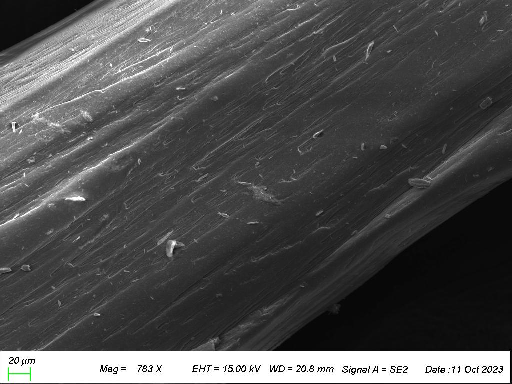
\includegraphics[width=0.46\textwidth]{bahiaGoeControl_20um4.pdf} &
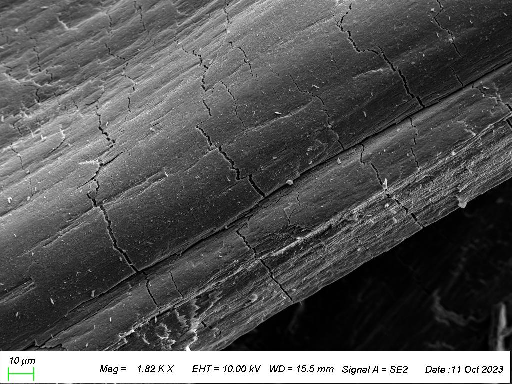
\includegraphics[width=0.46\textwidth]{Goethite_Vac_300C_11hr_10umB0.pdf} \\
\end{tabular}
\caption{Secondary electron images of Bahia goethite aggregate before heat treatment (control) and after heat treatment at 300\textdegree C for 11 hours in vacuum. Cracks developed in the vacuum-heated sample both parallel and perpendicular to the long axis of the polycrystalline aggregate, representing volume contraction due to dehydration/decomposition of goethite into hematite. The buffered treatments at the same temperature are shown in Fig.~\ref{fig:ch2-sem-buffered}.}
\label{fig:ch2-sem-control-vacuum}
\end{figure}

\begin{figure}[htbp]
\centering
\setlength{\tabcolsep}{4pt}
\begin{tabular}{cc}
\textbf{Gypsum-buffered, 300\textdegree C, 8 h} & \textbf{Water-buffered, 300\textdegree C, 4 h} \\[2pt]
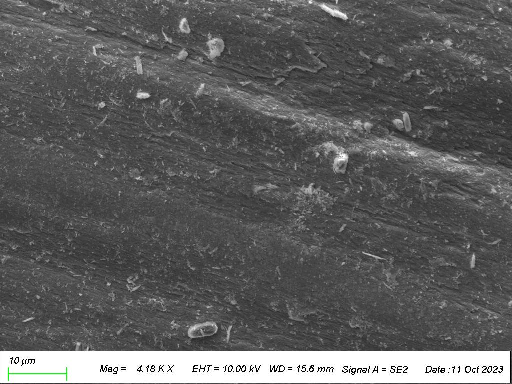
\includegraphics[width=0.46\textwidth]{bahiaGoeGypsum300C8hr_10um8.pdf} &
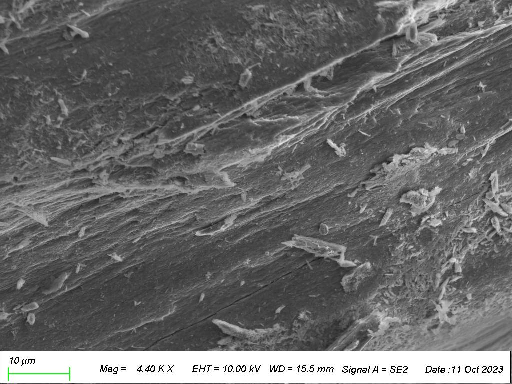
\includegraphics[width=0.46\textwidth]{Goeth_Water_300C_4hr_10um6.pdf} \\
\end{tabular}
\caption{Secondary electron images of Bahia goethite aggregate heated at 300\textdegree C in a sealed glass tube with gypsum (8 hours) and with water (4 hours). Despite treatment at high heat, no cracks indicative of dehydration were visible on either goethite surface. In the gypsum experiment, the gypsum dehydrated first and produced enough water pressure to stop or slow dehydration of the goethite and prevent the development of microscopic cracks; at higher temperatures goethite and gypsum reacted, forming a surface layer of other minerals. For the water-buffered sample, no cracks were observed when investigating the goethite at scales similar to Fig.~\ref{fig:ch2-sem-control-vacuum}, and most of the aggregate's surface resembled the gypsum-buffered panel; the area pictured had the roughest texture on the grain. A very small crack parallel to the long axis may indicate some amount of dehydration had occurred, or it could have been inherited from before hydrothermal treatment, since even the untreated control grain (Fig.~\ref{fig:ch2-sem-control-vacuum}) had some rough surfaces and rare long-axis-parallel cracks.}
\label{fig:ch2-sem-buffered}
\end{figure}

\begin{figure}[htbp]
\centering
\setlength{\tabcolsep}{4pt}
\begin{tabular}{cc}
\textbf{Vacuum, 300\textdegree C, 11 h (SE)} & \textbf{Vacuum, cross section (BSE)} \\[2pt]
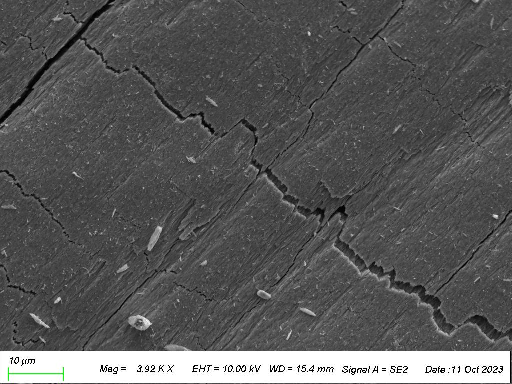
\includegraphics[width=0.46\textwidth]{Goethite_Vacuum_300C_11hr_10u9.pdf} &
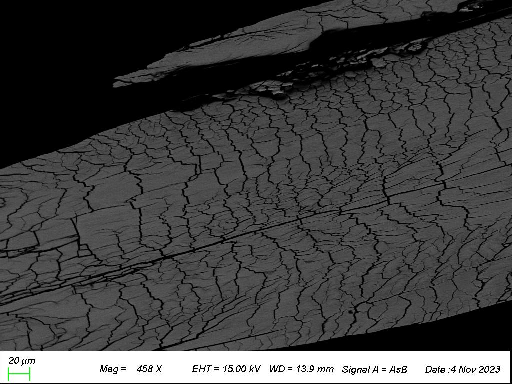
\includegraphics[width=0.46\textwidth]{C5_goeth_Vac205.pdf} \\
\end{tabular}
\caption{Vacuum-heated Bahia goethite at higher magnification and in cross section. Left: secondary electron image of goethite heated at 300\textdegree C for 11 hours in vacuum, at the same scale as the buffered samples of Fig.~\ref{fig:ch2-sem-buffered}, showing rough cracks at various scales both parallel and orthogonal to the long axis of the goethite aggregate. These are the typical decomposition features that would be expected in Fig.~\ref{fig:ch2-sem-buffered} if significant decomposition had occurred there. Right: backscatter electron image of a polished cross section of epoxy-mounted, vacuum-heated Bahia goethite, from the same subsample as the vacuum-heated grain of Fig.~\ref{fig:ch2-sem-control-vacuum}, exposing the grain's interior. This image clearly shows that the cracks visible on the exterior of dehydrated goethite are pervasive throughout the interior as well.}
\label{fig:ch2-sem-vacuum-interior}
\end{figure}

\section{Experimental Methods}\label{ch2-experimental-methods}

This study builds upon previous helium step heat studies of the dense
colloform goethite sample Win-06-01b (occasionally referred to as
Win0601b) collected within float at the Flinders Ranges in South
Australia \citep{waltenberg2012,monteiro2017}. It yields one of the
oldest known goethite U-Th/He ages: 180-135 Ma \citep{waltenberg2012}. To
produce a homogeneous distribution of 3He, Win-06-01b was irradiated
with 220 MeV protons for 24 hours at the Francis H. Burr Proton Therapy
Center, Massachusetts General Hospital, following standard procedures
\citep{shuster2005} and subsequently was subjected to helium step
heat measurements in vacuum by \citet{monteiro2017} and \citet{farley2024}.
In their step heat experiment of Win-06-01b, \citet{farley2024}
additionally measured evolved water using capacitance manometry to show
that helium and water release were tightly correlated for goethite step
heats in vacuum. Although they used subtly different heating schedules,
the results of \citet{farley2024} clearly agree well with \citet{monteiro2017}.

In this study, an aliquot of the same irradiated Win-06-01b goethite
used by \citet{monteiro2017} and \citet{farley2024} was encapsulated with
MilliQ water within a silica glass tube. Silica glass was chosen over
other laboratory glasses such as borosilicate because it is the most
permeable glass type to helium \citep{norton1953,altemose1961}. To
prepare the silica glass tube, 10 cm long segments of pure silica glass
tubes with an outer diameter of 4 mm and an inner diameter of 3 mm were
submerged and sonicated within acetone, ethanol, then MilliQ water baths
in sequence, and then were dried overnight in a 100°C oven. The glass
tubes were hand-pulled into thinner pipettes using a natural gas and
oxygen glass-welding torch and the pipette ends were fused closed. After
the glass had cooled, 1.18 mg of irradiated Win-06-01b goethite blades
less than 2 mm in length were carefully transferred to the bottom of the
tube in the presence of an ionizing fan. Less than a microliter of
distilled water was transferred to the sealed pipette using a thin glass
capillary, submerging the goethite, after which the tube was gently
tapped to liberate the bubbles and ensure that the water and goethite
were efficiently packed at the bottom of the pipette. To seal the
pipette, the contents of the ampoule were flash-frozen in liquid
nitrogen and transferred to a saltwater-ice bath at a temperature of
-10°C. While the pipette end of the tube remained frozen in the
saltwater-ice bath, the top was interfaced with a vacuum line and the
tube was pumped to a pressure of \textless0.1 torr. The advantage of
this approach was that water would remain solid within the tube, only
slowly sublimating to vacuum while atmospheric gasses would be readily
pumped away. While it was desirable to remove atmospheric gasses to
reduce experimental complexity by removing potentially reactive gasses
like oxygen, the primary motivation for pumping the tube to rough vacuum
was to aid the sealing process. When the tube contents were under
vacuum, fused glass would deform inwards and self-seal, greatly
improving the ease and quality of the seal while requiring far less heat
input from the torch. After an acceptably low pressure was attained, the
tube was closed to the vacuum line and the saltwater-ice bath was
quickly replaced with a liquid nitrogen bath, ensuring that no ice was
melted. The liquid nitrogen bath was preferable during sealing as it
more effectively protected the goethite and ice from the high
temperatures of the glass-welding torch. A fine-flamed welding torch was
used to seal the top of the ampoule, which dropped into the liquid
nitrogen bath and was retrieved by passing the liquid nitrogen through a
sieve. Fig.~\ref{fig:ch2-ampoule-post} shows the sealed ampoule after the completion of the
step heats with all of the original water remaining, a testament to the
quality of the ampoule's seal, which had sustained a massive pressure
gradient of over 11 orders of magnitude across the ampoule walls, with
an inner vapor pressure of about 3x10\textsuperscript{4} torr
(\textasciitilde40 bars: \citet{haar1984}) against the
\textasciitilde10\textsuperscript{-7} torr ultra-high vacuum of the lamp
cell while the ampoule was held at 250°C for over a week.

\begin{figure}[htbp]
\centering
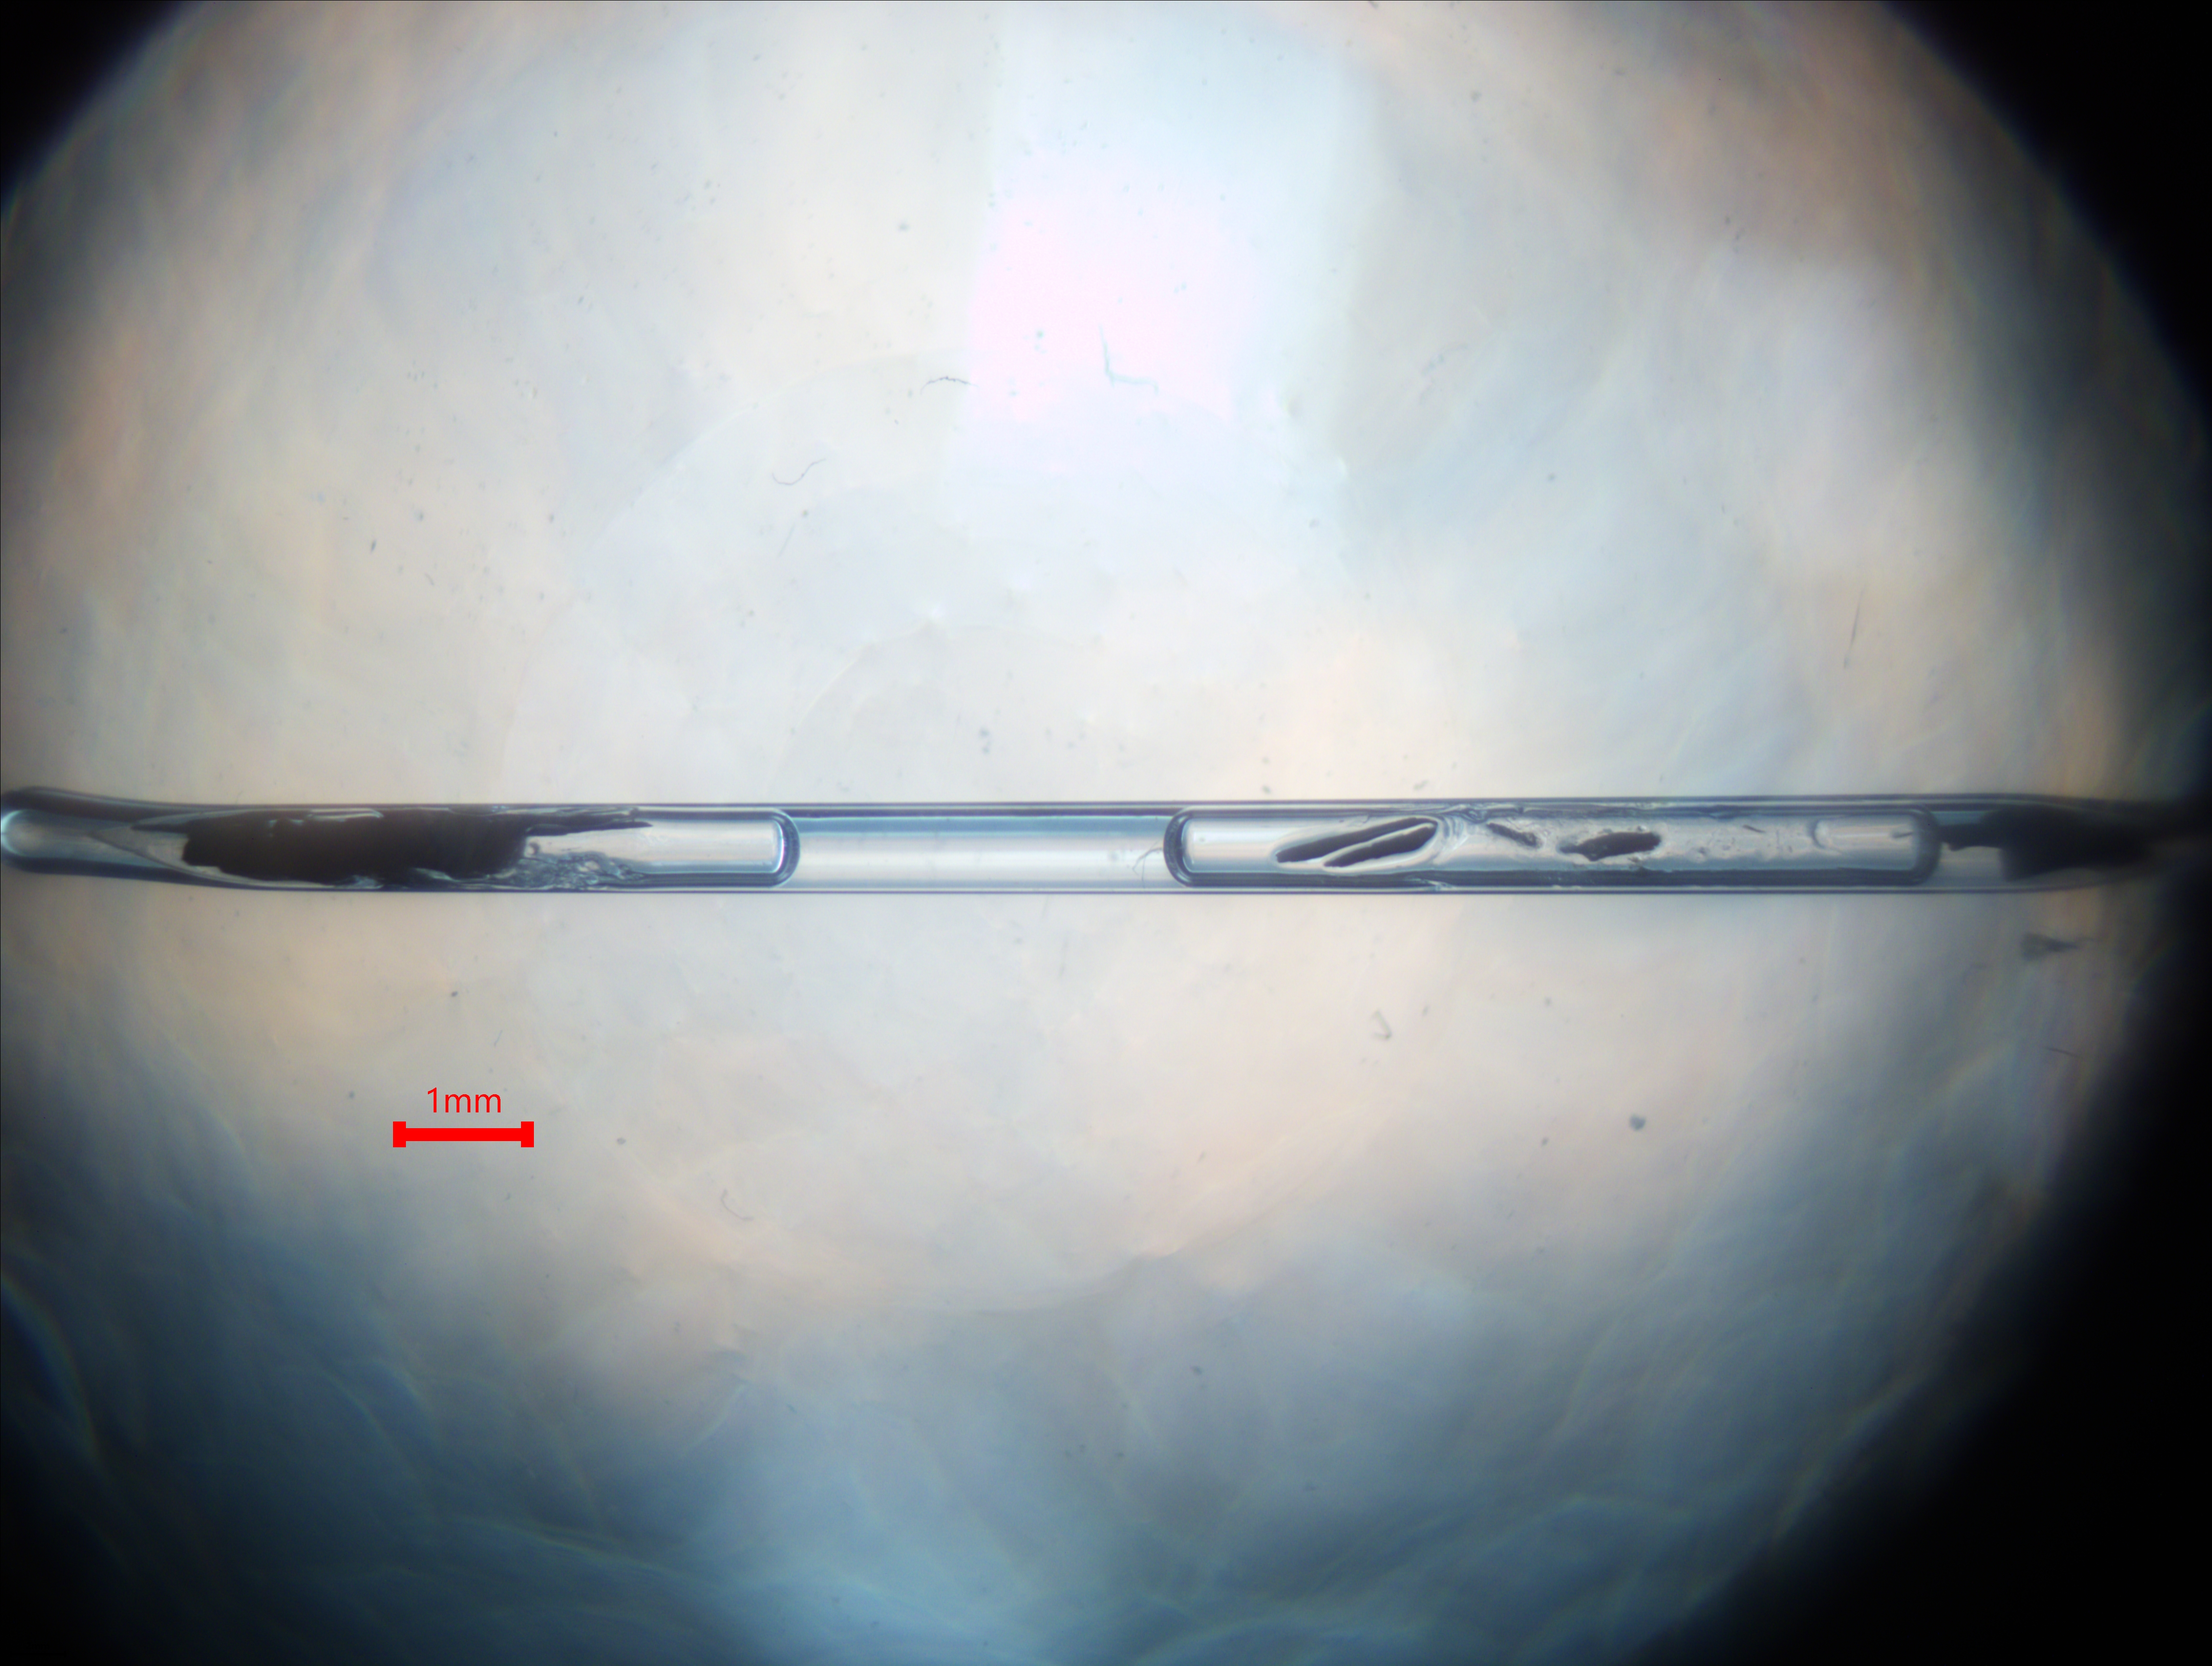
\includegraphics[width=0.7\textwidth]{zoomout2.jpg}
\caption{A view of the entire experimental ampoule after the completion of the step heat experiment before it was broken for the final step in the resistance furnace. At room temperature, the tube is approximately half-filled with gas, one-third filled with liquid water, and one-sixth filled with $<$2\,mm long shards of irradiated Win-06-01b goethite. A gel-like substance was observed lining the inner walls of the tube, which is likely to be amorphous silica dissolved from the tube and redeposited by the thermally-cycled, high pressure liquid water phase.}
\label{fig:ch2-ampoule-post}
\end{figure}

\begin{figure}[htbp]
\centering
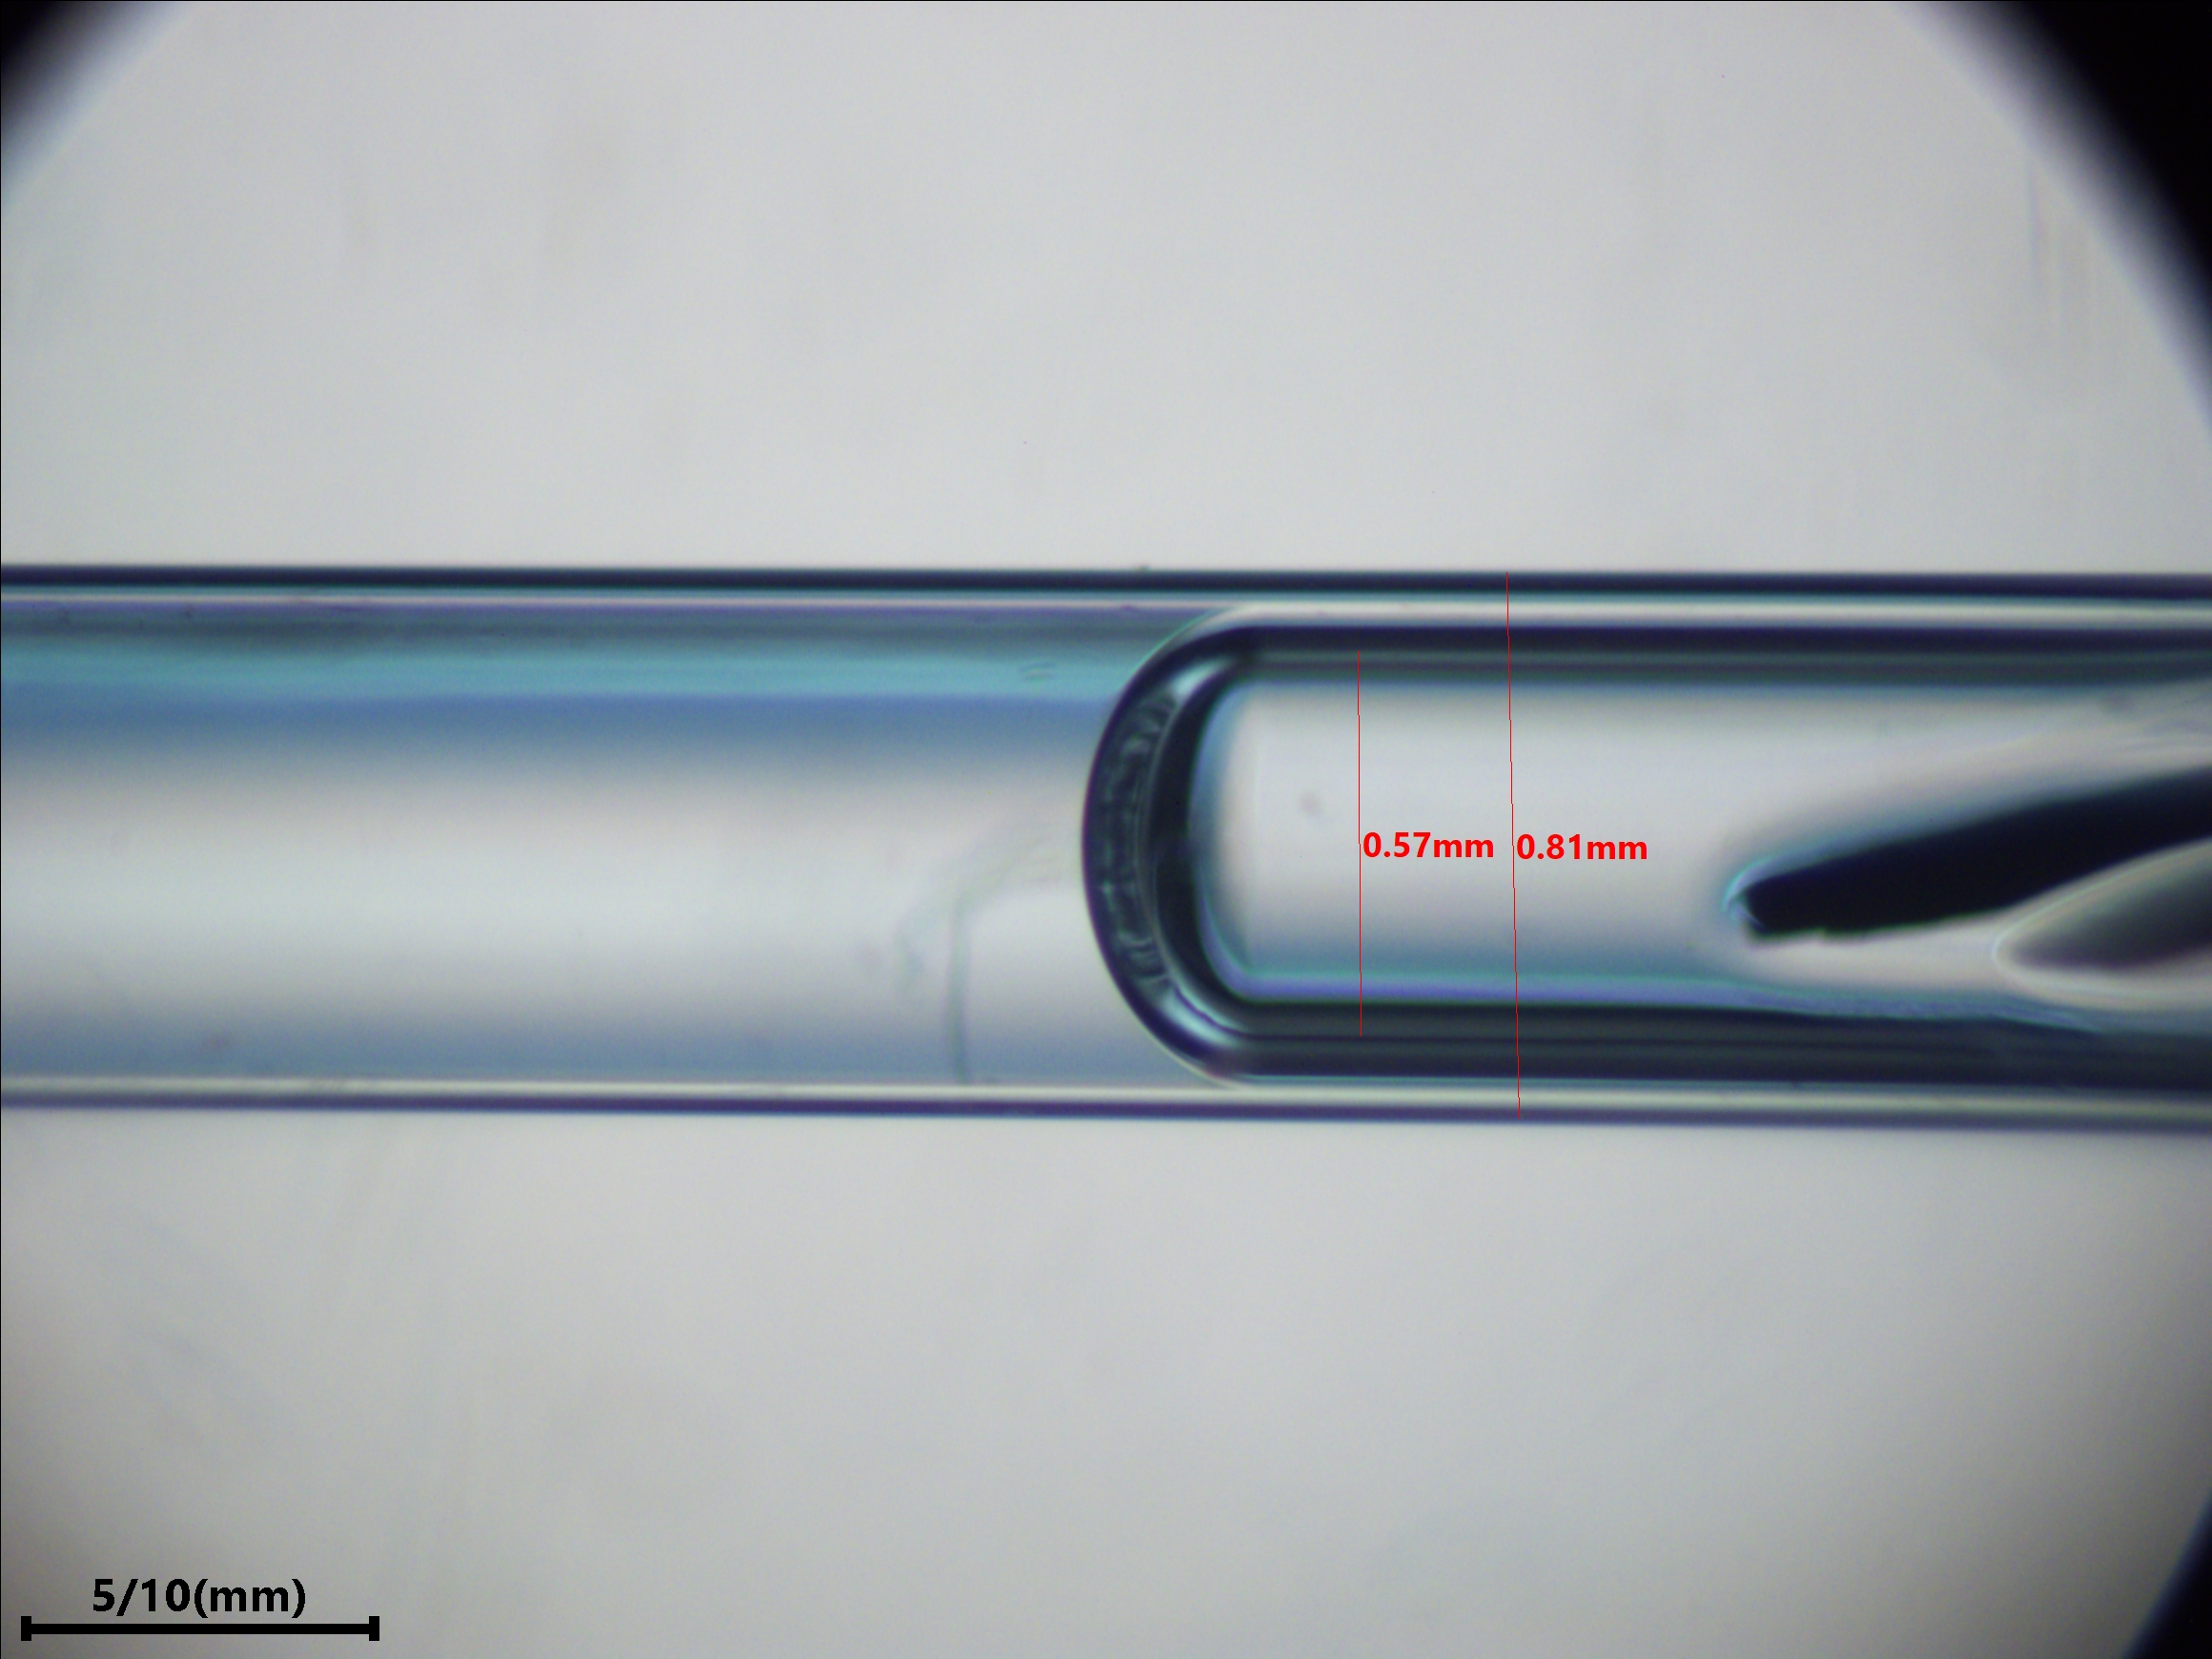
\includegraphics[width=0.7\textwidth]{measureGoeTube.jpg}
\caption{Measurements of the inner and outer diameter of the ampoule used in the hydrothermal step heats of Win-06-01b. The inner walls of the ampoule are only clearly visible within air bubbles.}
\label{fig:ch2-ampoule-dims}
\end{figure}

\clearpage


The sealed ampoule, now referred to as HT-Win-06-01b, was placed in a
copper foil packet and mounted to a K-type thermocouple within an
ultra-high vacuum projector lamp heating cell described in more detail
by \citet{farley1999}. Before the experiment began, the ampoule was
loaded in the lamp cell, pumped to high vacuum, and was held at 70°C for
4 days to degas atmospheric helium entrained within the ampoule.

HT-Win-06-01b was subjected to multiple prograde-retrograde heating
cycles to investigate possible MDD behavior. Step durations varied from
2 hours to about a week; the total experiment was conducted over about
40 days and included experimental steps ranging from 170-250°C. We
elected not to heat the sample hotter because high temperatures
generated very high vapor pressures. In early trials, we found that
similar ampoules most often withstood the \textasciitilde86 bar vapor
pressures associated with liquid water saturation at 300°C \citep{haar1984}, but they would explode when further heated to temperatures beyond
315°C.

Experimental temperature records show \textasciitilde1°C amplitude
oscillations around the target temperature. While we cannot exclude the
possibility that sustained temperature gradients were present throughout
the sample due to the use of the comparatively large \textasciitilde1 mm
thick ampoule, we are confident that the conclusions of this work are
robust. The ampoule was in direct contact with the thermocouple junction
and was in front of the thermocouple junction with respect to the projector
lamp heating source, suggesting that if there were a temperature
discrepancy, the sample would have been hotter than the recorded
temperature, which would not affect the conclusions of this work.
Additionally, during early trials of this method for helium step heats,
silica-glass encapsulated Durango apatite had been subjected to step
heats at Caltech and gave indistinguishable corrected 4He yields to
unencapsulated Durango apatite, suggesting that the temperature recorded
by the thermocouple for our experimental setup is sufficiently accurate.

Helium isotope measurements of evolved gasses from hydrothermal steps
heats of glass-encapsulated irradiated HT-Win-06-01b goethite were
acquired at Caltech on a Thermo Fisher
Helix-MC-Plus\textsuperscript{10K} mass spectrometer in peak hopping
mode from January 31\textsuperscript{st}, 2024 to March
13\textsuperscript{th}, 2024. Helium was purified by exposing evolved
gasses to a charcoal trap held in liquid nitrogen, a titanium sponge
getter, then a SAES NP10 getter before freely expanding into the
Helix-MC-Plus\textsuperscript{10K}. 3He was measured with a
pulse-counting electron multiplier, while 4He was detected on a Faraday
detector. The majority of the analysis time was spent measuring 3He.
Every few hours, the background was mass-scanned to set the 3He and 4He
measure points; each was taken to be a constant mass offset from the
background HD\textsuperscript{+} peak. These mass offsets are precisely
measured when tuning the Helix-MC-Plus\textsuperscript{10K} for helium
isotope analysis. Months of helium measurements with the
Helix-MC-Plus\textsuperscript{10K} at Caltech have shown this approach to
be reliable, reproducible, and accurate for helium isotope analysis.
Additionally, an electron multiplier monitored atomic mass 3.5 to detect
4He overspray, which was never significant during the experiment.
Measurements of high 3He MM gas standard were analyzed every 8 hours
(totaling 116 measurements) to track instrumental drift of 3He and 4He
sensitivities and to quantify internal reproducibility.

A cold blank was measured at the beginning of the experiment, showing a
negligible 3He blank essentially at 0 cps (technically this measurement
yielded a slightly negative intercept to time 0) and a 4He blank signal
corresponding to about 1.25 pccSTP, which was similar to 4He values
attained during low temperature permeation step measurements. Permeation
steps were thus assumed to measure shifting 4He blanks during the
experiment, and the entire blank correction was added to all 4He
uncertainties.

For the final step, the HT-Win-06-01b ampoule was broken and dried
overnight in a 50°C oven, then completely degassed by heating to
\textasciitilde1100 °C in a resistance furnace. The final step
measurement was conducted on a Thermo Fisher Helix SFT mass spectrometer. A
hot furnace blank subjected to the same volume splits as the final
HT-Win-06-01b measurement gave a 3He blank of 6.8 fccSTP and a 4He blank
of 0.31 nccSTP. This blank correction was less than 1\% of the measured
4He and negligible for 3He. A re-extract of HT-Win-06-01b immediately
following the measurement yielded above-blank 3He and 4He signals, which
were added to the total measurement, although both constituted less than
1\% of the final step yield. Sensitivity was calculated by measuring a
3He-enriched air standard with known 3He and 4He contents immediately
before the measurement.

Helium released by the sample reaches the mass spectrometer only after permeating the ampoule
wall, so each measured step yield lags the true release. Step yields were corrected for this
permeation lag with the bounding method of Chapter~\ref{ch:apparatus} (\S\ref{bounding-method}),
which gives lower-bound, central and upper-bound values for every step
(Tables~\ref{tab:ch2-distilled-3he} and~\ref{tab:ch2-distilled-4he}). The correction and the
ampoule permeabilities measured during the experiment are described in the Supplementary
Information (\S\ref{sec:ch2-si-permeation}), together with the diffusivity inversions, the
isotope-ratio uncertainties and the kinetic analysis of the published vacuum step heats
(\S\ref{ch2-analytical-methods}).

\paragraph{SEM Study of Thermally Treated Polycrystalline
Goethite}\label{sem-study-of-thermally-treated-polycrystalline-goethite}\label{sec:gt_pigment_methods}

In early trials of the ``glass tube method'' for helium step heat
experiments with controlled microenvironments presented here,
sub-samples of goethite morphologically similar to Win-06-01b from
Igarapé Bahia \citep{shustervasconcelos2005,monteiro2017} were heated in
vacuum using the projector lamp heating apparatus of \citet{farley1999}
and in sealed glass ampoules with gypsum or water additionally added to
provide moisture to slow/prevent dehydration of goethite. All samples
were held at 300°C for 4-11 hours, and the glass ampoules were broken
and the goethites were allowed to air dry before all samples were placed
on carbon tape and carbon coated. These samples were imaged at Caltech
on Secondary Electron mode by the ZEISS 1550VP Field Emission SEM.
Synthetic goethite pigment, a commercial yellow iron-oxide pigment of acicular crystals
$\sim$1~\textmu m long, was treated in the same way but only with water, without vacuum or
open-air runs: at least five larger silica glass ampoules, each loaded with pigment and an excess
of water and fused shut at ambient pressure, were held at 200--250~$^\circ$C for about a day in an
oven whose voltage was adjusted by hand. These runs were a rapid, qualitative test; details of
individual runs (temperature histories, durations, water-to-solid ratios) were not recorded, and
reaction was assessed by color (yellow goethite, red hematite) before imaging.
% TODO: add the pigment product name/grade and supplier; confirm SEM instrument/sample
% preparation for the pigment images (SE2, 10 kV, Feb 2024).

\section{\texorpdfstring{Results }{Results }}\label{ch2-results}

The complete corrected step-heat dataset underlying the diffusivities, delta plots, and Arrhenius regressions discussed below is distilled in Tables~\ref{tab:ch2-distilled-3he} and~\ref{tab:ch2-distilled-4he}, reporting the lower-bound, central, and upper-bound values from the bounding method's permeation-lag correction for $^3$He and $^4$He respectively.

\begin{landscape}
\begin{footnotesize}
\begin{longtable}{r r r r r r r r r r}
\caption{$^3$He step-heat dataset for HT-Win-06-01b under the bounding method: measured and cumulative $^3$He, the upper-bound residual ampoule content ($n_{t,\mathrm{UB}}$), the lower- and upper-bound true step production ($\omega_{\mathrm{LB}}$, $\omega_{\mathrm{UB}}$), and the corresponding lower-bound, central, and upper-bound apparent diffusivities. ``--'' denotes early steps with $\lambda t < 4$, for which bounds could not be determined (see \S\ref{permeation-lag-correction}). Six rows have derived values marked with ``*'': these steps have measured $^3$He $<0.1$ pccSTP and are excluded as low-signal from all plots (Fig.~\ref{fig:ch2-ratio-spectra} and others derived from this dataset).}\label{tab:ch2-distilled-3he}\\
\toprule
Temp & Time & $^3$He meas. & Cum. $^3$He & $n_{t,\mathrm{UB}}$ & $\omega_{\mathrm{LB}}$ & $\omega_{\mathrm{UB}}$ & $\ln(D/a^2)_{\mathrm{LB}}$ & $\ln(D/a^2)_{m}$ & $\ln(D/a^2)_{\mathrm{UB}}$ \\
(°C) & (min) & (pccSTP) & (pccSTP) & (pccSTP) & (pccSTP) & (pccSTP) &  &  &  \\
\midrule
\endfirsthead
\multicolumn{10}{l}{\textit{(continued)}} \\
\toprule
Temp & Time & $^3$He meas. & Cum. $^3$He & $n_{t,\mathrm{UB}}$ & $\omega_{\mathrm{LB}}$ & $\omega_{\mathrm{UB}}$ & $\ln(D/a^2)_{\mathrm{LB}}$ & $\ln(D/a^2)_{m}$ & $\ln(D/a^2)_{\mathrm{UB}}$ \\
(°C) & (min) & (pccSTP) & (pccSTP) & (pccSTP) & (pccSTP) & (pccSTP) &  &  &  \\
\midrule
\endhead
\midrule
\multicolumn{10}{r}{\textit{continued on next page}} \\
\endfoot
\bottomrule
\endlastfoot
170 & 300 & 0.9630 & 0.0000 & 1.1660 & -- & -- & -- & -- & -- \\
180 & 463 & 0.5442 & 0.9630 & 0.2413 & -- & -- & -- & -- & -- \\
190 & 550 & 0.5292 & 1.6241 & 0.1538 & -- & -- & -- & -- & -- \\
200 & 500 & 0.5190 & 2.2112 & 0.1430 & 0.3651 & 0.6619 & -22.158 & -21.775 & -21.503 \\
210 & 475 & 0.5770 & 2.7646 & 0.1440 & 0.4341 & 0.7210 & -21.715 & -21.406 & -21.160 \\
220 & 450 & 0.6333 & 3.3799 & 0.1447 & 0.4894 & 0.7781 & -21.345 & -21.068 & -20.843 \\
230 & 425 & 0.7899 & 4.0551 & 0.1685 & 0.6452 & 0.9584 & -20.823 & -20.604 & -20.392 \\
225 & 908 & 0.7513 & 4.8885 & 0.0716 & 0.5827 & 0.8229 & -21.516 & -21.246 & -21.148 \\
215 & 450 & 0.1415 & 5.6842 & 0.0349 & 0.0699 & 0.1764 & -22.836 & -22.124 & -21.900 \\
205 & 520 & 0.0763 & 5.8529 & 0.0184$^*$ & 0.0413$^*$ & 0.0947$^*$ & -23.479$^*$ & -22.863$^*$ & -22.646$^*$ \\
195 & 1106 & 0.0670 & 5.9491 & 0.0080$^*$ & 0.0487$^*$ & 0.0750$^*$ & -24.053$^*$ & -23.731$^*$ & -23.618$^*$ \\
185 & 740 & 0.0227 & 6.0246 & 0.0049$^*$ & 0.0147$^*$ & 0.0276$^*$ & -24.839$^*$ & -24.404$^*$ & -24.207$^*$ \\
175 & 920 & 0.0180 & 6.0610 & 0.0036$^*$ & 0.0131$^*$ & 0.0216$^*$ & -25.168$^*$ & -24.847$^*$ & -24.665$^*$ \\
200 & 260 & 0.0224 & 6.0814 & 0.0163$^*$ & 0.0189$^*$ & 0.0388$^*$ & -23.534$^*$ & -23.360$^*$ & -22.812$^*$ \\
210 & 520 & 0.0812 & 6.1081 & 0.0181$^*$ & 0.0649$^*$ & 0.0993$^*$ & -22.984$^*$ & -22.758$^*$ & -22.554$^*$ \\
220 & 1167 & 0.5766 & 6.1914 & 0.0447 & 0.5585 & 0.6213 & -21.587 & -21.553 & -21.475 \\
230 & 370 & 0.3577 & 6.7796 & 0.0903 & 0.3130 & 0.4480 & -20.948 & -20.811 & -20.579 \\
240 & 320 & 0.6767 & 7.1563 & 0.1776 & 0.5864 & 0.8543 & -20.062 & -19.913 & -19.667 \\
245 & 250 & 0.5549 & 7.8582 & 0.1888 & 0.3773 & 0.7437 & -20.176 & -19.778 & -19.474 \\
250 & 210 & 0.6934 & 8.4743 & 0.2786 & 0.5047 & 0.9721 & -19.626 & -19.296 & -18.942 \\
245 & 270 & 0.4659 & 9.2086 & 0.1413 & 0.1872 & 0.6071 & -20.801 & -19.874 & -19.601 \\
240 & 320 & 0.2857 & 9.7206 & 0.0749 & 0.1445 & 0.3606 & -21.176 & -20.487 & -20.250 \\
235 & 370 & 0.2199 & 10.0357 & 0.0517 & 0.1450 & 0.2716 & -21.284 & -20.864 & -20.650 \\
230 & 420 & 0.1400 & 10.2736 & 0.0303 & 0.0883 & 0.1703 & -21.885 & -21.421 & -21.224 \\
225 & 652 & 0.1494 & 10.4279 & 0.0206 & 0.1191 & 0.1700 & -22.009 & -21.781 & -21.650 \\
230 & 500 & 0.1550 & 10.5908 & 0.0271 & 0.1344 & 0.1820 & -21.605 & -21.462 & -21.299 \\
235 & 450 & 0.1951 & 10.7582 & 0.0361 & 0.1681 & 0.2313 & -21.258 & -21.107 & -20.936 \\
240 & 400 & 0.2425 & 10.9638 & 0.0483 & 0.2063 & 0.2908 & -20.913 & -20.750 & -20.566 \\
245 & 350 & 0.3150 & 11.2328 & 0.0690 & 0.2667 & 0.3840 & -20.495 & -20.326 & -20.125 \\
250 & 300 & 0.3716 & 11.5689 & 0.0939 & 0.3026 & 0.4656 & -20.181 & -19.973 & -19.743 \\
250 & 300 & 0.3640 & 11.9627 & 0.0899 & 0.2700 & 0.4539 & -20.261 & -19.959 & -19.734 \\
250 & 300 & 0.3452 & 12.3490 & 0.0852 & 0.2553 & 0.4304 & -20.285 & -19.979 & -19.755 \\
250 & 10250 & 8.4829 & 12.7167 & 0.0494 & 8.3977 & 8.5324 & -19.989 & -19.976 & -19.969 \\
240 & 785 & 0.2261 & 21.2187 & 0.0209 & 0.1767 & 0.2470 & -21.026 & -20.778 & -20.689 \\
\midrule
\textbf{Total} &  &  & 146.1483 &  &  &  &  &  &  \\
\end{longtable}
\end{footnotesize}
\end{landscape}

\begin{landscape}
\begin{footnotesize}
\begin{longtable}{r r r r r r r r r r r r r}
\caption{$^4$He step-heat dataset and absolute $^4$He/$^3$He ratios for HT-Win-06-01b under the bounding method, structured as in Table~\ref{tab:ch2-distilled-3he}. ``--'' denotes steps for which bounds could not be determined. The Total row reports the bulk (total-yield) $^4$He/$^3$He ratio, i.e. the normalizing value used to bulk-normalize these ratios for the plot in Fig.~\ref{fig:ch2-ratio-spectra}. Six rows have derived values marked with ``*'': these steps have measured $^3$He $<0.1$ pccSTP and are excluded as low-signal from all plots, as in Table~\ref{tab:ch2-distilled-3he}.}\label{tab:ch2-distilled-4he}\\
\toprule
Temp & Time & $^4$He meas. & Cum. $^4$He & $n_{t,\mathrm{UB}}$ & $\omega_{\mathrm{LB}}$ & $\omega_{\mathrm{UB}}$ & $\ln(D/a^2)_{\mathrm{LB}}$ & $\ln(D/a^2)_{m}$ & $\ln(D/a^2)_{\mathrm{UB}}$ & $(^4\mathrm{He}/^3\mathrm{He})_{\mathrm{LB}}$ & $(^4\mathrm{He}/^3\mathrm{He})_{m}$ & $(^4\mathrm{He}/^3\mathrm{He})_{\mathrm{UB}}$ \\
(°C) & (min) & (nccSTP) & (nccSTP) & (nccSTP) & (nccSTP) & (nccSTP) &  &  &  &  &  &  \\
\midrule
\endfirsthead
\multicolumn{13}{l}{\textit{(continued)}} \\
\toprule
Temp & Time & $^4$He meas. & Cum. $^4$He & $n_{t,\mathrm{UB}}$ & $\omega_{\mathrm{LB}}$ & $\omega_{\mathrm{UB}}$ & $\ln(D/a^2)_{\mathrm{LB}}$ & $\ln(D/a^2)_{m}$ & $\ln(D/a^2)_{\mathrm{UB}}$ & $(^4\mathrm{He}/^3\mathrm{He})_{\mathrm{LB}}$ & $(^4\mathrm{He}/^3\mathrm{He})_{m}$ & $(^4\mathrm{He}/^3\mathrm{He})_{\mathrm{UB}}$ \\
(°C) & (min) & (nccSTP) & (nccSTP) & (nccSTP) & (nccSTP) & (nccSTP) &  &  &  &  &  &  \\
\midrule
\endhead
\midrule
\multicolumn{13}{r}{\textit{continued on next page}} \\
\endfoot
\bottomrule
\endlastfoot
170 & 300 & 0.0192 & 0.0000 & 0.0280 & -- & -- & -- & -- & -- & -- & -- & -- \\
180 & 463 & 0.0305 & 0.0192 & 0.0152 & -- & -- & -- & -- & -- & -- & -- & -- \\
190 & 550 & 0.0558 & 0.0660 & 0.0179 & -- & -- & -- & -- & -- & -- & -- & -- \\
200 & 500 & 0.1024 & 0.1375 & 0.0313 & 0.0845 & 0.1337 & -26.207 & -25.965 & -25.619 & -- & 197.3 & -- \\
210 & 475 & 0.1460 & 0.2500 & 0.0404 & 0.1147 & 0.1864 & -25.314 & -25.022 & -24.717 & 248.2 & 253.0 & 268.8 \\
220 & 450 & 0.2091 & 0.4055 & 0.0530 & 0.1686 & 0.2620 & -24.407 & -24.152 & -23.876 & 326.3 & 330.1 & 349.3 \\
230 & 425 & 0.3243 & 0.6319 & 0.0760 & 0.2714 & 0.4004 & -23.425 & -23.213 & -22.956 & 403.7 & 410.6 & 432.3 \\
225 & 908 & 0.3483 & 0.9799 & 0.0363 & 0.2722 & 0.3845 & -23.807 & -23.527 & -23.413 & 442.6 & 463.6 & 474.4 \\
215 & 450 & 0.0716 & 1.3487 & 0.0196 & 0.0353 & 0.0912 & -24.945 & -24.225 & -23.976 & 429.1 & 505.9 & 537.1 \\
205 & 520 & 0.0385 & 1.4359 & 0.0103$^*$ & 0.0189$^*$ & 0.0487$^*$ & -25.661$^*$ & -24.942$^*$ & -24.701$^*$ & 392.4$^*$ & 504.2$^*$ & 534.6$^*$ \\
195 & 1106 & 0.0336 & 1.4912 & 0.0043$^*$ & 0.0233$^*$ & 0.0379$^*$ & -26.165$^*$ & -25.796$^*$ & -25.675$^*$ & 446.7$^*$ & 500.9$^*$ & 515.3$^*$ \\
185 & 740 & 0.0079 & 1.5467 & 0.0019$^*$ & 0.0037$^*$ & 0.0098$^*$ & -27.586$^*$ & -26.808$^*$ & -26.592$^*$ & 224.7$^*$ & 350.1$^*$ & 369.1$^*$ \\
175 & 920 & 0.0152 & 1.6020 & 0.0033$^*$ & 0.0133$^*$ & 0.0185$^*$ & -26.475$^*$ & -26.340$^*$ & -26.141$^*$ & 843.2$^*$ & 843.2$^*$ & 982.0$^*$ \\
200 & 260 & 0.0107 & 1.6351 & 0.0091$^*$ & 0.0073$^*$ & 0.0198$^*$ & -25.787$^*$ & -25.411$^*$ & -24.791$^*$ & 375.6$^*$ & 475.5$^*$ & 554.7$^*$ \\
210 & 520 & 0.2166 & 1.6547 & 0.0535$^*$ & 0.2075$^*$ & 0.2701$^*$ & -23.067$^*$ & -23.021$^*$ & -22.786$^*$ & 2667.1$^*$ & 2667.1$^*$ & 3103.8$^*$ \\
220 & 1167 & 0.3187 & 1.8714 & 0.0269 & 0.2652 & 0.3456 & -23.499 & -23.302 & -23.214 & 471.7 & 552.7 & 563.2 \\
230 & 370 & 0.2113 & 2.6766 & 0.0590 & 0.1844 & 0.2703 & -22.391 & -22.249 & -21.993 & 575.1 & 590.8 & 628.0 \\
240 & 320 & 0.4286 & 3.1616 & 0.1243 & 0.3697 & 0.5529 & -21.360 & -21.203 & -20.931 & 612.1 & 633.4 & 674.8 \\
245 & 250 & 0.3988 & 3.6430 & 0.1521 & 0.2746 & 0.5510 & -21.289 & -20.899 & -20.556 & 665.9 & 718.7 & 778.4 \\
250 & 210 & 0.4440 & 4.2359 & 0.2020 & 0.2918 & 0.6460 & -20.906 & -20.469 & -20.072 & 541.7 & 640.2 & 702.8 \\
245 & 270 & 0.3123 & 4.7263 & 0.1053 & 0.1103 & 0.4176 & -22.043 & -20.981 & -20.680 & 469.1 & 670.4 & 721.4 \\
240 & 320 & 0.1927 & 5.0846 & 0.0559 & 0.0874 & 0.2485 & -22.376 & -21.575 & -21.315 & 505.5 & 674.3 & 718.4 \\
235 & 370 & 0.1517 & 5.3031 & 0.0393 & 0.0958 & 0.1910 & -22.386 & -21.922 & -21.688 & 599.8 & 689.6 & 729.9 \\
230 & 420 & 0.0991 & 5.4714 & 0.0236 & 0.0598 & 0.1227 & -22.956 & -22.448 & -22.232 & 608.3 & 707.9 & 745.9 \\
225 & 652 & 0.0995 & 5.5835 & 0.0151 & 0.0760 & 0.1146 & -23.136 & -22.863 & -22.721 & 608.2 & 666.5 & 689.2 \\
230 & 500 & 0.1051 & 5.6969 & 0.0202 & 0.0900 & 0.1253 & -22.679 & -22.523 & -22.345 & 652.1 & 678.1 & 707.5 \\
235 & 450 & 0.1369 & 5.8251 & 0.0279 & 0.1167 & 0.1648 & -22.290 & -22.128 & -21.940 & 674.6 & 701.7 & 734.0 \\
240 & 400 & 0.1781 & 5.9762 & 0.0390 & 0.1502 & 0.2171 & -21.892 & -21.719 & -21.518 & 705.1 & 734.6 & 770.9 \\
245 & 350 & 0.2305 & 6.1807 & 0.0556 & 0.1915 & 0.2861 & -21.479 & -21.290 & -21.070 & 694.4 & 731.9 & 771.7 \\
250 & 300 & 0.2777 & 6.4385 & 0.0758 & 0.2221 & 0.3535 & -21.134 & -20.906 & -20.659 & 703.3 & 747.3 & 793.3 \\
250 & 300 & 0.2654 & 6.7374 & 0.0725 & 0.1896 & 0.3379 & -21.250 & -20.908 & -20.661 & 653.7 & 729.2 & 774.1 \\
250 & 300 & 0.2489 & 7.0231 & 0.0680 & 0.1764 & 0.3169 & -21.282 & -20.932 & -20.647 & 646.8 & 721.0 & 765.4 \\
250 & 10250 & 6.8042 & 7.2901 & 0.0430 & 6.7362 & 6.8472 & -20.704 & -20.691 & -20.682 & 800.6 & 802.1 & 803.3 \\
240 & 785 & 0.1853 & 14.1156 & 0.0187 & 0.1423 & 0.2040 & -21.688 & -21.422 & -21.325 & 770.5 & 819.4 & 838.0 \\
\midrule
\textbf{Total} &  &  & 145.8145 &  &  &  &  &  &  &  & 997.7 &  \\
\end{longtable}
\end{footnotesize}
\end{landscape}


The diffusivities determined from the corrected step heat 3He and 4He
yields for HT-Win-06-01b are always significantly lower than the
diffusivities determined from step heat experiments on the same sample
in vacuum, and evolutions that are distinct from those determined from
the vacuum experiments. The Arrhenius plot of the 3He diffusivities
initially follow a declining concave-up trend until \textasciitilde3.5\%
cumulative 3He yield, then slowly decreasing in sub-parallel arrays
during prograde and retrograde heating cycles from 3.5-7\% cumulative
3He yields (Fig.~\ref{fig:ch2-arrhenius-zoom}, Fig.~\ref{fig:ch2-delta-zoom}). The Arrhenius plot of the 4He diffusivities
differs in shape: it is concave-down to about 5\% cumulative 3He yield,
after which it follows a roughly linear array about one log unit below
the 3He array (Fig.~\ref{fig:ch2-arrhenius-zoom}). The 3He diffusivities settled into a
linear array which was suitable for linear regression after
\textasciitilde7\% of the cumulative 3He yield was lost (Fig.~\ref{fig:gt_arrhenius}b). All
remaining diffusivity measurements of the experiment were included in
the linear regression, so that diffusivities from 3He loss fractions of
about 7-15\% were included. The linear regression yields an
R\textsuperscript{2} of \ChTwoRtwo, an activation energy of \ChTwoEa ± \ChTwoEaErr
kJ/mol, and a closure temperature of \ChTwoTc ± \ChTwoTcErr °C assuming a cooling
rate of 10°C/Ma and considering only the uncertainty in the regression
intercept (D\textsubscript{0}/a\textsuperscript{2}).
\begin{figure}[htbp]
\centering
\includegraphics[width=\textwidth]{arrhenius_reaction_vs_diffusion.pdf}
\caption{The $^3$He release of every step of the two vacuum step heats of Win-06-01b (red circles:
KAF, \citealt{farley2024}; orange squares: HDM, \citealt{monteiro2017}) and of the hydrothermal
step heat of this study (blue diamonds), reduced in two ways: (a) as first-order conversion rate
constants $k_i$ (Eq.~\eqref{eq:gt_stepk}, $\phi=\ChTwoKinPhi$), and (b) as \citet{fechtigkalbitzer1966}
apparent diffusivities $D/a^2$ for a sphere (Eq.~\eqref{eq:gt_FK}). The points of each experiment
are joined in step order by dashed lines. Filled vacuum symbols are the steps in the kinetic fitting
window and open symbols lie outside it; large pink circles mark the two KAF steps with the
LN$_2$ trap isolated. Hydrothermal steps are bounding-method central values, with bars spanning the
lower and upper bounds; low-signal steps are excluded. Black line: joint first-order Arrhenius fit
to the KAF and HDM steps in the window (Eq.~\eqref{eq:gt_line}). The two reductions give the
experiments opposite geometries. For the vacuum step heats, the first-order reduction collapses
both heating schedules onto one line, including the retrograde steps of HDM, whereas the diffusion
reduction separates the schedules, places HDM's retrograde steps above its own prograde steps and
turns over above $\sim$275~$^\circ$C as release stalls at the hematite plateau, none of which a
depleting diffusion domain can produce. For the hydrothermal step heat the pattern reverses. As rate
constants, its steps sit 1.3--2.8 orders of magnitude below the vacuum line and split into
history-dependent arrays that first-order kinetics forbids, with retrograde steps below prograde
steps at the same temperature. As diffusivities, the same steps form a single coherent array,
approximately seven natural-log units below the vacuum values, whose offsets through the temperature
cycles follow the depletion of the least retentive domains (\S\ref{sec:gt_hydro}). Below
$\sim$180~$^\circ$C both vacuum experiments depart from the first-order line, reflecting a small,
separate low-temperature component (\S\ref{sec:gt_vacuum}). Steps with $F>1-\phi$ have no defined
$k$ and are absent from (a).}
\label{fig:gt_arrhenius}
\end{figure}

\begin{figure}[htbp]
\centering
\includegraphics[width=0.8\textwidth]{winsor_goethite_Diffusivities_Arrhenius_Zoomin.pdf}
\caption{Linear regression of the last \ChTwoN\ measurements of 3He diffusivities in HT-Win-06-01b defining the ``Stage 1'' reference line. Apparent diffusivities under hydrothermal conditions are approximately seven natural log units lower than in vacuum. A diffusion domain corresponding to the Stage 1 reference line has a closure temperature of \ChTwoTc$\pm$\ChTwoTcErr\textdegree C assuming a cooling rate of 10\textdegree C/Ma. Apparent diffusivities calculated from 4He step heats are sometimes within error of those calculated for 3He, however they are occasionally resolved at the 2$\sigma$ level and are about a single log unit lower than apparent diffusivities calculated for 3He after a cumulative fractional yield of 14\% 3He.}
\label{fig:ch2-arrhenius-zoom}
\end{figure}

\clearpage


A delta plot was generated using the intercept and slope parameters from
the 3He regression as a reference line, similarly to previous work
\citep{farley2018}. The 3He apparent diffusivity delta values monotonically
decrease until a cumulative 3He loss of 7\%, after which the delta
values are within error of Delta = 0: the reference line (Fig.~\ref{fig:ch2-delta-zoom}). A
series of low-yield measurements on the first retrograde cycle produce
high-error diffusivities which appear as scattered, uncertain delta
values just after a cumulative 3He loss of 4\% for both 3He and 4He.
\begin{figure}[htbp]
\centering
\includegraphics[width=0.8\textwidth]{DeltasWinsorGTzoomin_VacuumHydrothermal.pdf}
\caption{Delta plot similar to those presented in \citep{farley2018}, or r/r0 plots in \citet{lovera1991} and \citet{farleyflowers2012}. Delta plots are the difference between apparent log diffusivities and a reference line; they are designed to remove the temperature dependence of the dominant process of helium migration to reveal how apparent diffusivities evolve as an experiment proceeds. Each step is drawn as a bar spanning its starting to ending cumulative 3He fractional yield; hydrothermal bars span each step's uncertainty with the central value marked, vacuum steps are drawn as lines at their delta values, and thin vertical lines join adjacent steps. For visual continuity, the gap left by excluded hydrothermal steps is bridged by extending the preceding step's central value across its first half and the following step's across its second half; no uncertainty is shown over the bridge. 3He monotonically decreases until settling on a temporary plateau from 4--6\% 3He fractional yield, then settling on the reference line from 7--15\% 3He fractional yield, which is consistent with MDD systematics. 4He diffusivities and delta values are generally highly uncertain but initially show an increase in delta values that settles to a slow increase or plateau about one log unit below the 3He reference line by a 3He fractional yield of 5\%, which is consistent with diffusive loss of radiogenic 4He in the least retentive domains interrogated in HT-Win-06-01b. Apparent diffusivities for helium in Win-06-01b in hydrothermal conditions are up to 7 log units lower than the same sample in vacuum.}
\label{fig:ch2-delta-zoom}
\end{figure}

\section{Discussion}\label{ch2-discussion}

\paragraph{Consistency with MDD
Systematics}\label{consistency-with-mdd-systematics}

Previous work on helium step heats of goethite in vacuum have
demonstrated degassing behavior in the laboratory that is inconsistent
with thermally activated volume diffusion through goethite. For example,
apparent diffusivities calculated from helium step heat experiments of
goethites with uniform distributions of 3He produced by proton
irradiation following the methods of \citet{shuster2004} will increase
in an isothermal experiment \citep{farley2024}, which is inconsistent
with volume diffusion through an unchanging crystal.

\citet{farley2024} reported that helium and water evolution in goethite
vacuum step heating experiments are highly correlated and concluded that
the crystal was decomposing into water and hematite during the
experiment.

The goal of this work was to attempt to slow this decomposition process
below the rate of thermal helium loss in unchanging goethite. SEM
imagery shows that goethite that is thermally treated when encapsulated
with water (or gypsum) does not extensively dehydrate like
goethite heat-treated in vacuum or open air (Figs.~\ref{fig:ch2-sem-control-vacuum}--\ref{fig:ch2-sem-vacuum-interior}). While it is
difficult to prove that decomposition or recrystallization is not
playing a role in the results presented in this work, the apparent
diffusivities observed for the Win-06-01b goethite under hydrothermal
conditions are much lower than those observed in previous step heats of
Win-06-01b in vacuum (Fig.~\ref{fig:gt_arrhenius}b, Fig.~\ref{fig:ch2-arrhenius-zoom}, Fig.~\ref{fig:ch2-delta-zoom}, Fig.~\ref{fig:ch2-isothermal-retention}), implying that
processes other than dehydration may be responsible for the observed
apparent diffusivities. This is tested quantitatively in
\S\ref{sec:gt_vacuum}--\ref{sec:gt_hydro}, and explained in \S\ref{sec:gt_nucleation}.

All helium step heat data on goethites are from naturally occurring
polycrystalline aggregates with unclear and potentially widely variable
grain sizes \citep{monteiro2017,farley2024}, which are expected to
follow MDD systematics. If volume diffusion is responsible for the data
reported here, they too would be expected to follow MDD systematics. In
MDD systems, apparent bulk diffusivities of a homogeneously distributed
diffusant at a single temperature will decrease as an experiment
proceeds, as would delta or r/r0 values at any temperature (where
\(\Delta = \ ln\left( \frac{D}{a^{2}} \right)_{measured} - ln\left( \frac{D}{a^{2}} \right)_{reference}\)
) \citep{lovera1991,farley2018}, assuming that the activation
energy of the reference line used in such plots matches that of the
process controlling diffusion. For the activation energy of \ChTwoEa{}~kJ/mol
retrieved by regression in this work, the homogeneously distributed 3He
step heat data follow the expected MDD systematics and monotonically
decrease within a delta plot (Fig.~\ref{fig:ch2-delta-zoom}), which is consistent with
volume diffusion in a MDD system.

The strong plateau in the delta plot and statistically robust regression
over a wide range of fractional cumulative 3He yield (from 7-15\% $\Sigma F_{3\mathrm{He}}$
with an R\textsuperscript{2} of \ChTwoRtwo) suggests that the frequency
factor obtained by the regression may be dominated by a particular
diffusion domain, rather than a mix of diffusion domains as is most
often observed in the apparent diffusivities for polycrystalline
hematite \citep{farley2018}. The 4He apparent diffusivities are generally
lower than the 3He apparent diffusivities and increased at the beginning
of the experiment, which is consistent with rounding of 4He
concentration profiles due to loss of radiogenic helium in the least
retentive domains \citep{shuster2004,shustervasconcelos2005}.

Many vacuum experiments in goethite also record declining delta values
for early fractional yields of 3He \citep{shustervasconcelos2005,farley2024} that are generally not represented in the 4He data. This effect
may be from helium migrating out of fast pathways along grain boundaries
that would retain little helium in nature \citep{shustervasconcelos2005}.
Goethite aggregates are known to have interstices that are filled by
chemisorbed non-stoichiometric water that represents the earliest water
to be lost in vacuum \citep{naono1987}. Non-stoichiometric hydrogen
is known to persist in goethite even after heating to 140°C \citep{yapppoths1995}. It is therefore reasonable to posit that artificial 3He
observed in less-retentive domains may be trapped by non-stoichiometric
water or hydroxyl groups within interstices of goethite aggregates.
Dehydration of non-stoichiometric interstitial water may be associated
with early fractions of degassing water and 3He from goethite samples
during step heats, and could potentially represent the LRD (low retention
domain) of \citet{shustervasconcelos2005}, and the 3He offgassed during ``Stage
1'' in vacuum step heats \citep{farley2024}. The high variability of
the portion of 3He hosted in early-degassing ``Stage 1'' fractions
within vacuum step heats is sensible considering observations that
goethite formed at different temperatures is known to have highly
variable crystallinity, crystallite ordering, surface area, and
non-stoichiometric water contents \citep{schwertmann1985}. This
population of 3He would likely also be the first to be lost under
hydrothermal conditions.

While the results presented here are strong experimental evidence for
high helium retentivity in goethite (Fig.~\ref{fig:ch2-isothermal-retention}, Fig.~\ref{fig:ch2-fourier-hematite-ref}), they do not yet
independently provide any evidence to support or refute hypotheses that
helium diffusion in crystalline goethite is anisotropic or affected by
radiation damage \citep{bassal2022}.

\paragraph{Vacuum Step Heats of Win-06-01b Are Controlled by Conversion to Hematite}\label{sec:gt_vacuum}

Fitting the first-order conversion model of \S\ref{sec:gt_kinetics_methods}
(Eqs.~\eqref{eq:gt_Fphi}--\eqref{eq:gt_F1_cum}) to the cumulative KAF $^3$He
release by least squares gives $E_a = \ChTwoKinFOneEa$~kJ\,mol$^{-1}$, $\ln A = \ChTwoKinFOneLnA$ ($A$ in s$^{-1}$),
$\phi = \ChTwoKinPhi$ and $s = \ChTwoKinS$, with an rms misfit in $F$ of \ChTwoKinFOneRmsKAF{} over the
\ChTwoKinNKAF{} steps of the fitting window (\S\ref{sec:gt_kinetics_methods}). The step rate constants of
both experiments (Eq.~\eqref{eq:gt_stepk}) fall on a single Arrhenius line
(Fig.~\ref{fig:gt_arrhenius}a). This includes the HDM retrograde steps, which a first-order
process requires: its rate depends only on $T$ and on the amount of goethite remaining. An
unweighted least-squares fit of $\ln k_i$ against $1/T_i$ for the \ChTwoKinLineN{} steps in the fitting window
gives
\begin{equation}
  E_a = \ChTwoKinLineEa \pm \ChTwoKinLineEaErr~\mathrm{kJ\,mol^{-1}},
  \qquad
  \ln A = \ChTwoKinLineLnA \pm \ChTwoKinLineLnAErr
  \label{eq:gt_line}
\end{equation}
(KAF alone $\ChTwoKinKAFEa\pm\ChTwoKinKAFEaErr$; HDM alone $\ChTwoKinHDMEa\pm\ChTwoKinHDMEaErr$~kJ\,mol$^{-1}$), in agreement with the
cumulative fit. At 250~$^\circ$C this gives $k = \ChTwoKinKTwoFifty$~s$^{-1}$, or \ChTwoKinConvPerHour\% conversion
per hour. The result does not depend on the fitting window: fitting all steps instead gives
$E_a = \ChTwoKinAllFOneEa$~kJ\,mol$^{-1}$ and the same ranking of models (\S\ref{sec:gt_supp_mech}).
Thermogravimetric studies of goethite dehydroxylation report somewhat higher apparent activation
energies, $154\pm15$ to $169\pm8$~kJ\,mol$^{-1}$, for a reaction controlled by a two-dimensional
phase boundary, with a different mechanism at early stages and low temperature \citep{goss1987}.
% TODO: compare conditions (heating in air/N2 vs vacuum; sample grain size) before finalizing.

In the diffusion representation (Fig.~\ref{fig:gt_arrhenius}b) the two experiments do not
collapse. HDM's retrograde steps between 180 and 220~$^\circ$C plot about three natural-log units
above HDM's own prograde steps at the same temperatures. Volume diffusion from grains that are
being progressively depleted cannot produce this, whether from a single domain or multiple
domains: retrograde steps must fall on or below the prograde trend. $D/a^2$ also turns over
above $\sim$275~$^\circ$C, where release stalls at the plateau.

The kinetic rate parameters fitted to KAF alone predict the independent HDM schedule with an rms misfit in
$F$ of \ChTwoKinFOneRmsHDM{} over the fitting window. A single-domain spherical diffusion model fits KAF worse
(rms \ChTwoKinDThreeRmsKAF) and predicts HDM worse (rms \ChTwoKinDThreeRmsHDM). It also predicts $F\to1$ by
$\sim$300~$^\circ$C, whereas both experiments stall at $F\approx0.89$. Giving the diffusion model the
same hematite-inherited fraction as the first-order fit ($\phi = \ChTwoKinPhi$), and fitting the same
steps, lowers its misfit to KAF to \ChTwoKinDThreePhiRmsKAF, still \ChTwoKinDThreePhiRmsRatio{} times that
of the first-order model, but does not improve its prediction of HDM (rms \ChTwoKinDThreePhiRmsHDM), and it
requires $E_a = \ChTwoKinDThreePhiEa$~kJ\,mol$^{-1}$. Leaving $\phi$ free
($\phi = \ChTwoKinDThreeFreePhi$) gives \ChTwoKinDThreeFreeRmsKAF{} and \ChTwoKinDThreeFreeRmsHDM
(Table~\ref{tab:gt_mech_fits}). Within a single schedule, fits alone cannot discriminate
between kinetic mechanisms (\S\ref{sec:gt_supp_mech}). The second schedule is what gives the
comparison its power.

% NOTE: remove this paragraph if 4He/3He is to be avoided entirely
During the main vacuum release (KAF, $0.04<F<0.88$), the step $^4$He/$^3$He ratio stays within
0.95--1.10 of the bulk ratio. Grains therefore release their integrated inventory as they
convert, rather than releasing a diffusive, rim-weighted component.

In both experiments release stalls at $F\approx0.89$. The fitted $\phi=\ChTwoKinPhi$ is the same for KAF
and HDM. In HDM, the remaining $\sim$\ChTwoKinPhiPct\% is released slowly between 340 and 500~$^\circ$C and on
fusion. We interpret this fraction as $^3$He inherited by the hematite product and subsequently
released by the much slower diffusion out of hematite. Single-domain goethite diffusion cannot
produce a plateau. The conversion and the plateau correspond to the ``Stage 2'' and
``Stage 3'' release of \citet{farley2024}, whose transition near $F\approx0.88$ is independent of
heating schedule (Fig.~\ref{fig:ch2-delta-zoom}).

In two KAF steps the trap was isolated and evolved water accumulated in the line. At
230~$^\circ$C the step rate constant fell to \ChTwoKinTrapSuppLow{} times the mean of its neighbors at the same
temperature, and at 240~$^\circ$C to \ChTwoKinTrapSuppHigh{} times. The rate recovered fully when the trap was
restored. Water and $^3$He were suppressed together. A diffusion process would not respond to
the partial pressure of water. We return to these two steps in \S\ref{sec:gt_nucleation}, where
they calibrate the nucleation model.

Below $\sim$180~$^\circ$C both vacuum experiments release $^3$He 0.5--3 orders of magnitude
faster than the extrapolated conversion rate (Fig.~\ref{fig:gt_arrhenius}). This component amounts
to less than 2\% of the $^3$He and is not conversion. We attribute it to diffusion from the least
retentive domains (\S\ref{consistency-with-mdd-systematics}).

\paragraph{Helium Release under Hydrothermal Conditions Is Diffusive}\label{sec:gt_hydro}

The hydrothermal experiment heated an aliquot of the same goethite in distilled water, with
much of the sample submerged in the liquid. The schedule rose from 170 to 230~$^\circ$C, cycled
down to 175~$^\circ$C, rose to 250~$^\circ$C, cycled down to 225~$^\circ$C and back to 250~$^\circ$C,
where three 5~h steps preceded a 170.8~h step, and ended with a step at 240~$^\circ$C (442.8~h in
total). Only 14.7\% of the $^3$He was released. Under the vacuum kinetics of
Eq.~\eqref{eq:gt_line}, the same schedule would have converted the sample completely. Two tests,
both applied to the bounding-method reduction (Table~\ref{tab:ch2-distilled-3he}), show that the
release follows diffusion rather than conversion.

\textit{Test 1: history dependence through temperature cycles.} A line through the first
prograde sweep (200--230~$^\circ$C) serves as the reference. The two retrograde steps of the
first cycle with adequate signal, at 225 and 215~$^\circ$C, fall 0.45 and 0.86 natural-log units
below it in $\ln(D/a^2)$ (Eq.~\eqref{eq:gt_FK}; central values). The upper bound of each step
still falls 0.18 and 0.47 log units below a line fitted to the lower bounds of the first sweep.
On the next prograde sweep, the 220~$^\circ$C step sits 0.58 log units (at least 0.32) below its
first-sweep value (Fig.~\ref{fig:gt_arrhenius}b). The low-signal steps of the first
retrograde sweep (205--175~$^\circ$C, and 200--210~$^\circ$C on the following prograde sweep;
excluded from all plots) sit lower still, by 1.3--2.1 log units. In the last cycle, retrograde and
prograde values at 230--245~$^\circ$C agree within 0.07--0.45 log units, and their bounds
overlap at every temperature. The Stage 1 regression over this interval (cumulative yield
$\geq$7\%) gives $E_a = \ChTwoEa\pm\ChTwoEaErr$~kJ\,mol$^{-1}$
(\S\ref{helium-in-goethite-diffusivity-inversions}). This is the signature of depleting fast,
low-retentivity domains in the first cycle, with diffusion dominated by more retentive domains
thereafter. A first-order conversion rate depends only on temperature and on the fraction
converted, which is almost unchanged at $F\approx0.04$. It would return retrograde steps to the
prograde line, as the vacuum HDM experiment does in the reaction representation
(Fig.~\ref{fig:gt_arrhenius}a).

\textit{Test 2: the 250~$^\circ$C holds.} The two processes project differently through a long
isothermal step. Diffusion slows as the diffusion front moves inward, whereas first-order
conversion proceeds at a nearly constant rate while $\alpha\ll1$. We calibrate both on the three
5~h steps at 250~$^\circ$C and project through the 170.8~h step. For first-order conversion,
$-\ln(1-\alpha)$ grows linearly in time at fixed $T$ (Eq.~\eqref{eq:gt_F1}), so
\begin{equation}
  F(t) = (1-\phi)\left[1-(1-\alpha_0)\,e^{-kt}\right],
  \qquad \alpha_0 = \frac{F_0}{1-\phi},
\end{equation}
with $k$ fitted to the three calibration steps and $F_0 = 0.0795$ (bounds 0.0793--0.0798) the
release before the first of them. For diffusion from a sphere, the Fourier number $Dt/a^2$ grows
linearly in time at fixed $T$:
\begin{equation}
  F(t) = 1 - \frac{6}{\pi^2}\sum_{n=1}^{\infty}\frac{1}{n^2}
  \exp\!\left[-n^2\pi^2\left(\left(\frac{Dt}{a^2}\right)_0 + \frac{D}{a^2}\,t\right)\right],
\end{equation}
where $(Dt/a^2)_0$ follows from $F_0$ by Eq.~\eqref{eq:gt_FK} and $D/a^2$ is fitted to the
calibration steps. Both models reproduce the three calibration steps (Fig.~\ref{fig:gt_hold}).
Over the long step they diverge. Diffusion projects $F = 0.149$ against an observed 0.146
(bounds 0.1460--0.1463). First-order conversion projects 0.173, overpredicting the release in
that step by 46\%: $(0.173-0.087)/(0.146-0.087) = 1.46$. Calibrating instead on the lower- and
upper-bound series gives 0.148--0.150 for diffusion and 0.172--0.174 (a 44--47\%
overprediction) for first-order conversion. We also tested the contracting-geometry and Avrami
models of \S\ref{sec:gt_supp_mech}, which fit the vacuum data less well. Calibrated the same
way, they project 0.174--0.212, and none changes the result.

\begin{figure}[htbp]
  \centering
  \includegraphics[width=0.65\linewidth]{hydrothermal_hold_projection.pdf}
  \caption{The 250~$^\circ$C holds of the hydrothermal experiment. Black: observed cumulative
  $^3$He fraction (bounding-method central values; bars span the lower and upper bounds).
  Curves: first-order conversion and spherical volume diffusion, each calibrated on the three
  5~h steps (grey band) and projected through the 170.8~h step; faint bands show the same
  projections calibrated on the lower- and upper-bound series.}
  \label{fig:gt_hold}
\end{figure}

Plotted as first-order rate constants (Fig.~\ref{fig:gt_arrhenius}a), the hydrothermal steps sit
1.3--2.8 orders of magnitude (median 2.4) below the vacuum line. They show what a first-order
process forbids: retrograde steps 0.7--1.5 natural-log units below prograde steps at the same
temperature, and a falling $k$ during the 250~$^\circ$C holds. In the diffusion representation
(Fig.~\ref{fig:gt_arrhenius}b) the same steps form a coherent, history-dependent array. The
vacuum experiments behave like conversion and the hydrothermal experiment behaves like
diffusion. Section~\ref{sec:gt_nucleation} shows that these observations require the conversion
rate at water saturation to be at least $10^{2.5}$ times slower than in vacuum, and that every
water-inhibition law consistent with both data sets predicts far more suppression than that.

% -----------------------------------------------------------------------------

\paragraph{Goethite Dehydration and/or Recrystallization During
Helium Step Heat
Experiments}\label{goethite-dehydration-andor-recrystallization-during-hydrothermal-experiments}

The aim of helium step heat experiments is to characterize the
mechanisms and rates helium loss in nature to aid in the interpretation
of geochronologic and helium geochemical data. While the results of this
experiment are encouraging in that they differ remarkably from
experiments on the same and similar samples in vacuum that are primarily
controlled by dehydration processes \citep{farley2024}, this
experiment may also be affected to some degree by processes aside from
volume diffusion that may potentially be unrelated to helium loss in
goethite in nature.

Aside from nanoparticles \citep{guobarnard2011,navrotsky2008}, bulk goethite is unstable with respect to hematite and water at
the pressures and temperatures of this experiment \citep{majzlan2003} (\S\ref{sec:gt_thermo}). The SEM study of goethite heat-treated in vacuum and open air shows that clearly visible volume contraction cracks
form throughout the interiors and surfaces of highly-dehydrated goethite grains, while goethite heat-treated in water-saturated conditions
does not (Figs.~\ref{fig:ch2-sem-control-vacuum}--\ref{fig:ch2-sem-vacuum-interior}).
Clearly, dehydration is occurring at a much smaller scale, if at all, in the hydrothermal experiments. While this evidence excludes the possibility of pervasive dehydration in
the hydrothermal experiments, it does not exclude the possibility of some dehydration occurring at a scale too small to be observed in the SEM images. Future work
on textural evolution of natural goethite aggregates during low fraction dehydration would be useful to resolve the extent of ``hidden'' dehydration that may occur before
the formation of SEM-visible cracks.

The kinetic analysis of \S\ref{sec:gt_vacuum}--\ref{sec:gt_hydro}, and the nucleation analysis of
\S\ref{sec:gt_nucleation}, indicate that solid-state dehydration contributed negligibly to the helium loss of Win-06-01b-HT: at water
saturation, every water-inhibition law consistent with the vacuum and hydrothermal data slows
conversion by about five orders of magnitude or more (Table~\ref{tab:gt_ratelaws}), and the release shows the history and time dependence of diffusion rather than
conversion. If dehydration nevertheless contributed to the helium loss of Win-06-01b-HT, the new
data presented here would represent upper
bounds for the apparent diffusivities of helium at the temperatures and
fractional cumulative yields ($\Sigma F_{\mathrm{He}}$).

The process of recrystallization is another potential complication in
interpreting helium step heats of goethite in hydrothermal conditions.
Poorly crystalline synthetic goethite held in hydrothermal conditions is
known to recrystallize into more orderly, crystalline goethite
aggregates, even at temperatures as low as 125°C in as little as 16
hours \citep{schwertmann1985}. In this study, natural goethite was
held in contact with liquid water and water vapor at hydrothermal
conditions as harsh as \textasciitilde40 bars and 250°C for as long as a
week. These conditions appear to have visibly dissolved and
reprecipitated silica from the ampoule's inner walls (Fig.~\ref{fig:ch2-ampoule-post}),
qualitatively testifying to the ability of the hydrothermal fluid to
dissolve and recrystallize rock-forming oxides. It is unquestionable
that recrystallization of some goethite could have occurred under these
conditions; however, it is unclear if conditions were favorable to
recrystallize this specimen of goethite, Win-06-01b, which is amongst
the most helium-retentive and crystalline dated goethite samples
\citep{waltenberg2012,farley2024}. Less crystalline goethites in
nature are commonly recrystallized, which appears to result in helium
loss, resetting the U-Th/He age \citep{monteiro2018,monteiro2014,heim2006}. Intuitively, it is difficult to imagine that
dissolution-precipitation mediated recrystallization would not result in
complete loss of helium within recrystallized regions. Therefore,
assuming an initially uniform distribution of 3He throughout the crystal
from proton irradiation, the upper bound extent of recrystallization
would be equivalent to the 3He cumulative fractional yield, which is
only 14.7\% by the end of the hydrothermal experiment. Remaining helium is
unlikely to pass through these now helium-free recrystallized areas if
grain boundaries in goethite serve as fast pathways like they do in
hematite \citep{farley2018}. Recrystallization could be the dominant process
controlling helium loss in this experiment, but only if it is faster
than diffusive loss, in which case the data presented here would
represent new upper bounds for apparent diffusivities for helium in
Win-06-01b goethite. In that case, it stands to reason that processes
such as dehydration and recrystallization may be faster than volume
diffusion of helium in crystalline goethite in nature and may be the
primary drivers of helium loss.


% --- Added 2026-09-25 (goethite stability integration; see CHANGES_JOURNAL.md) ---
\paragraph{Fluid-Mediated Conversion of Synthetic Goethite Pigment}\label{sec:gt_pigment}

Goethite can also convert to hematite through the fluid, by dissolution of goethite and
precipitation of hematite, and this fluid-mediated conversion does occur in some materials. In the
qualitative experiments on
acicular synthetic goethite pigment (\S\ref{sec:gt_pigment_methods}), heated with excess water at
200--250~$^\circ$C for about a day, the outcome was all or nothing. Roughly equal proportions of
ampoules were completely reacted (red), completely unreacted (yellow), or contained both
reacted and unreacted material. In the mixed ampoules, the red and yellow portions were entirely
isolated from one another, separated by gas bubbles. Unreacted pigment retains its acicular habit
(Fig.~\ref{fig:gt_pigment}b). The reacted product is instead composed of equant to platy crystals
$\sim$0.5--1~\textmu m across (Fig.~\ref{fig:gt_pigment}a), interpreted as hematite from its color
and habit. The change of shape rules out pseudomorphic dehydroxylation. It indicates dissolution of
goethite and nucleation and growth of hematite from the fluid, a pathway outside the solid-state
nucleation model developed in \S\ref{sec:gt_nucleation}.

\begin{figure}[htbp]
  \centering
  \begin{subfigure}[t]{0.48\textwidth}
    \centering
    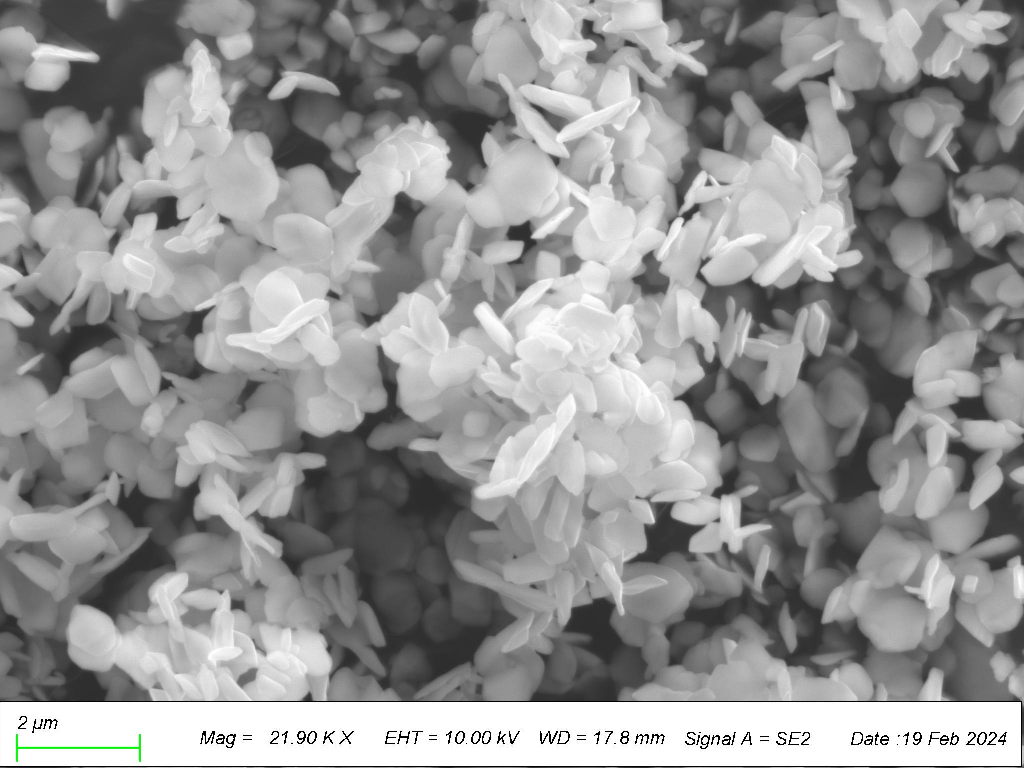
\includegraphics[width=\textwidth]{goe_pig_treatedRed19.pdf}
    \caption{Reacted (red) product}
    \label{fig:gt_pigment_red}
  \end{subfigure}\hfill
  \begin{subfigure}[t]{0.48\textwidth}
    \centering
    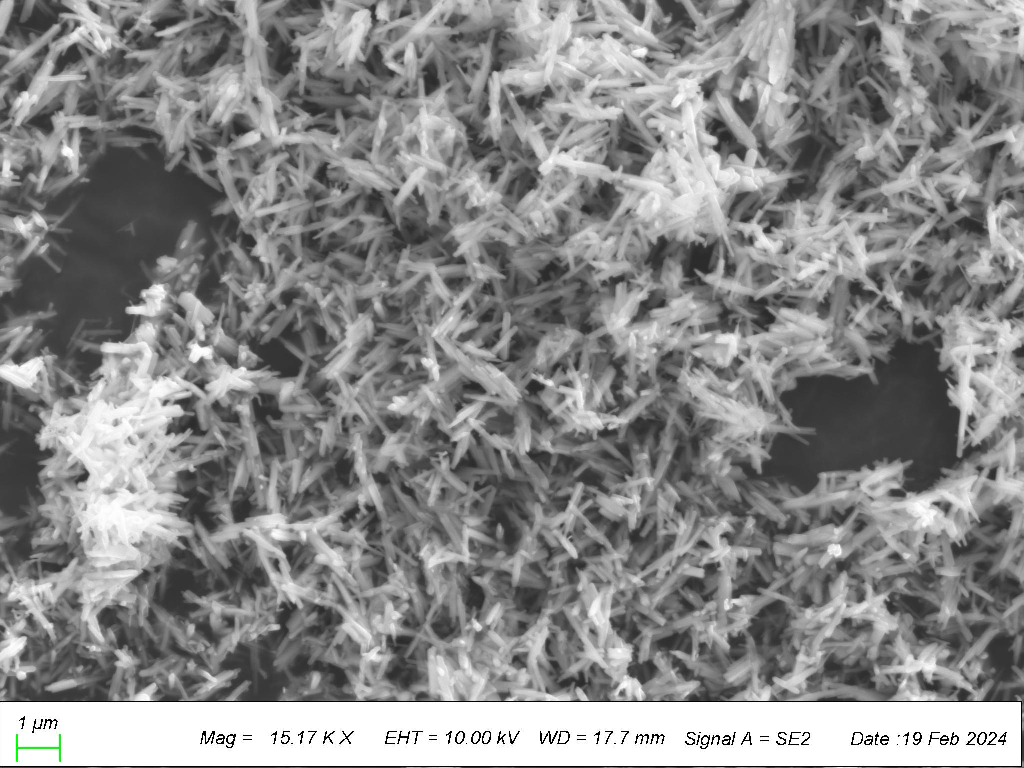
\includegraphics[width=\textwidth]{goe_pig_treatedYellow37.pdf}
    \caption{Unreacted (yellow) pigment}
    \label{fig:gt_pigment_yellow}
  \end{subfigure}
  \caption{Secondary electron images of synthetic goethite pigment after hydrothermal treatment
  at 200--250~$^\circ$C for about a day (\S\ref{sec:gt_pigment_methods}). (a) Material from a
  completely reacted (red) ampoule: the acicular goethite has been replaced by equant to platy
  crystals $\sim$0.5--1~\textmu m across, interpreted as hematite. (b) Material from an
  unreacted (yellow) ampoule, which retains the acicular habit of the starting pigment. The change
  in crystal habit requires dissolution of goethite and precipitation of hematite from the fluid,
  and the all-or-nothing outcome of the experiments indicates that the reaction is limited by
  nucleation and proceeds rapidly once it begins.}
  \label{fig:gt_pigment}
\end{figure}

The distribution of outcomes is itself diagnostic. Conversion either went to completion within
a fluid-connected volume or did not occur at all, even where reacted and unreacted pigment shared
the same ampoule and thermal history. This is the behavior of a nucleation-limited process:
once hematite nucleates, the reaction proceeds rapidly to completion, and where it does not
nucleate, goethite persists for the full run. The fluid-mediated pathway is therefore governed,
like the solid-state pathway, by the difficulty of forming a hematite nucleus rather than by the
rate at which hematite grows.

We conclude that water-saturated conditions do not by themselves exclude fluid-mediated
conversion of goethite, even where solid-state conversion is suppressed (\S\ref{sec:gt_nucleation}). Whether that pathway operates
depends on the solution chemistry. For the natural sample in distilled water,
\S\ref{sec:gt_hydro} shows that the release is diffusive; a nucleation-limited, all-or-nothing
reaction would also be expected to release helium abruptly rather than in the smooth,
history-dependent manner observed. For samples whose chemistry is less well characterized, the
absence of conversion should be verified directly, for example by post-run X-ray diffraction or
electron microscopy.

\paragraph{\texorpdfstring{High Helium Retentivity of
Win-06-01b-HT}{ High Helium Retentivity of Win-06-01b-HT}}\label{high-helium-retentivity-of-win-06-01b-ht}

Apparent diffusivities calculated from helium step heats on the
hydrothermal experiment on Win-06-01b goethite are clearly resolved and
much lower than the apparent diffusivities calculated for the same
sample in vacuum by \citet{monteiro2017} and \citet{farley2024} for all steps
after the first few (Fig.~\ref{fig:gt_arrhenius}b, Fig.~\ref{fig:ch2-arrhenius-zoom}, Fig.~\ref{fig:ch2-delta-zoom}). Diffusivities calculated
from the hydrothermal experiment are approximately seven natural log
units lower than the earlier experiments in vacuum on the same sample. This high
helium retentivity is explored through three lenses: closure temperature
of cooling samples \citep{dodson1973}, isothermal diffusion \citep{wolf1998}, and through comparison with step heats of other polycrystalline
samples. Strictly speaking, both closure temperatures and retention
estimations under isothermal diffusion only apply to helium loss
occurring exclusively via thermally activated volume diffusion with
known domain size. While the results presented here on a polycrystalline
sample are consistent with a thermally activated volume diffusive
process for helium loss in goethite under hydrothermal conditions, they
do not exclude other processes (such as goethite
dehydration/decomposition/recrystallization) or potential complexities
related to radiation damage and crystal defects on bulk diffusion
\citep{bassal2022}, nor do they permit estimation of the diffusivity
at infinite temperature (D0).

If the slope and intercept on the regression of 3He apparent
diffusivities from this experiment are taken to represent a real
diffusion domain for goethite, then a closure temperature can be
calculated for this domain. Considering uncertainty only in the
intercept (D\textsubscript{0}/a\textsuperscript{2}) term and a cooling rate of 10°C/Ma, the closure
temperature for that domain would be \ChTwoTc ± \ChTwoTcErr °C.

Goethite is formed near Earth's surface and thus U-Th/He geochronology
is most typically applied to date surface processes \citep{heim2006,yappshuster2011,vasconcelos2013,danisik2013,monteiro2014,hofmann2017,allard2018}. For
crystals of goethite grown near the surface that are found near the
surface, the concept of a closure temperature is poorly applicable, as
it necessarily assumes a cooling rate \citep{dodson1973}. In such cases, a
better measure of retentivity is an analysis of isothermal retentivity
over time \citep{wolf1998}, which is commonly expressed in terms of
t'/t, where t' is the helium age and t is the isothermal holding time
(most often the `real age'). For an isothermal holding time of 100 Ma at
40°C, a diffusive domain with the parameters obtained from the
regression of 3He apparent diffusivities of Win-06-01b-HT has a t'/t = 0.968, where t'/t = 1 corresponds to perfect retentivity. Fig.~\ref{fig:ch2-isothermal-retention}
shows isothermal holding time against helium age for this same domain
for 4 different temperatures. At 25°C, this domain is nearly
quantitatively retentive of helium even at billion-year time scales. The
results presented here qualitatively support that goethite is highly
retentive of helium at surface conditions, even at 100-million-year
timescales.
\begin{figure}[htbp]
\centering
\includegraphics[width=0.8\textwidth]{PRP_goethite_winsor.pdf}
\caption{Isothermal retention plot \citep{wolf1998} for helium in goethite corresponding to the ``Stage 1'' reference line regression on the hydrothermal experiment. Helium hosted in a diffusion domain with these diffusion parameters would be nearly perfectly retentive at billion-year timescales at 25\textdegree C. At 40\textdegree C, the equilibrium age for this domain (the helium age at which radiogenic helium production and diffusive loss are equal) is 33.2 billion years, attained after 50.4 billion years.}
\label{fig:ch2-isothermal-retention}
\end{figure}

It is difficult to use Arrhenius plots to compare many samples' helium
retentivities. \citet{farley2024} report that linear regressions on
apparent diffusivities calculated from helium step heat data on goethite
in vacuum can be fit to yield widely variable diffusive parameters even
for a single sample (e.g. activation energies ranging from 107 to 176
kJ/mol within a single experiment on YAN-0201 AC). Similarly,
regressions on helium step heat data of polycrystalline materials can
yield erroneous activation energies when not applied carefully \citep{farley2018}. Because of the complexity of comparing Arrhenius plots of
calculated apparent diffusivities for polycrystalline samples with
differing heating schedules, it is advantageous to convert heating
schedules to some parameter that can be compared easily between
experiments. One effective way to reduce the complexity of step heat
experiments to visualize helium retentivity is to ``flatten'' a thermal
history to a dimensionless diffusive timescale: the Fourier number (Fo =
Dt/a\textsuperscript{2}). This approach offers similar benefits to Delta plots
\citep{farley2018} or r/r0 plots \citep{lovera1991}, but is optimized to
qualitatively compare the helium retentivities of polycrystalline
samples for a given thermal history (expressed as diffusive time).

For a given diffusive domain, a Fourier number of Fo $\approx$ 1 corresponds to
the complete degassing of that domain. Complex heating schedules can be
converted to Fourier numbers by assuming a reference line similarly to a
Delta or r/r0 plot \citep{lovera1991,farley2018}. This procedure
is especially useful for MDD (Multiple Diffusion Domain) systems, where
the apparent diffusivities decrease over the course of a step heat
experiment as the least retentive domains are degassed. For a single
spherical diffusion domain, the fraction of helium released is a
function of the Fourier number alone \citep{crank1979,fechtigkalbitzer1966}. If the activation energy of the reference
Fourier number is the same as the activation energy of diffusion, then
the amount of helium released in that domain then is an exact function
of the reference Fourier number multiplied by a constant. Thus, a plot
with reference Fourier numbers against cumulative fractional helium
yields for different samples will yield the same geometries and
interrelationships regardless of the intercept used to calculate the
reference Fourier numbers; the values of the reference Fourier numbers
will be arbitrary and only meaningful as relative diffusive time.
Another implication is that different aliquots of the same sample should
appear identical in this space regardless of heating schedule (see the vacuum step heats of
Win-06-01b and the overlapping hematite samples in Fig.~\ref{fig:ch2-fourier-hematite-ref}).
Many such plots were generated with a variety of activation energies between
149 kJ/mol to 171 kJ/mol, but the relative positions of the degassing curves for all samples are preserved, 
illustrating the utility of this approach even for comparing helium retentivity between different minerals. 

Fig.~\ref{fig:ch2-fourier-hematite-ref} compares the step heat results of Win-06-01b-HT with 11
step heat experiments of 3 samples of polycrystalline hematite and 9
step heat experiments of 2 samples of goethite in Vacuum, including
Win-06-01b. In a thermal-history normalized space, it is obvious that
goethite in vacuum and hematite define well-separated populations and
goethite in vacuum is far less retentive of helium than hematite. Most
interestingly, the most retentive sample on these plots is clearly the
Win-06-01b-HT goethite under water-saturated conditions, at least for the
14.7\% of the total 3He hosted in the least retentive domains. This plot shows
that step heat results for different, unrelated goethite samples in vacuum are more similar to one
another than step heat results of the same sample at different water
activities.
\begin{figure}[htbp]
\centering
\includegraphics[width=0.75\textwidth]{Fo_Plot_hematite_ref_HematiteGoethite.pdf}
\caption{Heating schedules for polycrystalline goethite and hematite samples are flattened to reference Fourier numbers, dimensionless numbers that can be thought of as integrated thermal history, allowing for easy comparison of entire helium step heat experiments. The 3He cumulative fractional yield is plotted on the $y$ axis as a function of Fourier number in log scale on the $x$ axis. Curves on the left of the plot degas earlier within a given thermal history than the curves on the right. Hematite and goethite step heats in vacuum each cluster closely together, forming distinct populations. Most strikingly, the hydrothermal Win-06-01b-HT experiment is the most helium-retentive polycrystalline sample on the plot, at least until the experiment's end at a cumulative fractional yield $\sim$15\% F3He. In vacuum, all hematite samples are significantly more retentive of helium than all goethite samples, with some limited exceptions for the least retentive domains holding $<$5\% of the total helium. Win-06-01b step heat experiments in vacuum are indistinguishable from the Capao samples in vacuum (the two leftmost goethites are Capao samples; the rest of the Capao samples closely cluster with Win-06-01b in vacuum). The differences in the curves here reflect differences in grain size distributions for hematite, and some combination of grain size and dehydration rate (due to variable water pressure in the experimental vessel and crystal aggregate size) for goethite. Vacuum step heats of 11 aliquots of 4 samples of polycrystalline hematite from the Grand Canyon, Arizona \citep{farleyflowers2012} and the Gogebic Range, Michigan \citep{farleymckeon2015}, and 9 aliquots of Win-06-01b and Capao goethite from Minas Gerais, Brazil \citep{monteiro2017,farley2024} are plotted here. The reference $D/a^2$ values are calculated for 1\textmu m domains of hematite (ln($D_0$) = 0.66; $E_a$ = 171 kJ/mol: \citep{farley2018}), and the reference curve for the degassing of 1\textmu m spherical domains of hematite with uniformly distributed 3He is calculated using the forward equations of \citet{fechtigkalbitzer1966}.}
\label{fig:ch2-fourier-hematite-ref}
\end{figure}

\paragraph{Profiling Radiogenic Helium Loss with $\frac{^4He}{^3He}$ Ratios of Win-06-01b-HT}\label{spectra-of-win-06-01b-ht}

Bulk-normalized 4He/3He ratios in step heats of irradiated samples
measure rounding concentration profiles by natural helium loss, if the
loss mechanism in nature and in the laboratory share the same geometry
\citep{shuster2004,farley2024}. Aside from the first
experimental step, bulk-normalized 4/3 ratios for all experiments begin
at vanishingly small values and steeply increase at first, with the rate
of increase slowing as the experiments proceed (Fig.~\ref{fig:ch2-ratio-spectra}). This
behavior is consistent with complete then partial loss of radiogenic
helium in nature in the least retentive domains and is observed in all
step heat experiments on irradiated goethite \citep{farley2024}. The
hydrothermal experiment, however, records lower bulk-normalized 4/3
ratios than the vacuum experiments at any given $\Sigma F_{3\mathrm{He}}$ for the duration
of the experiment. Similarly, the approach to the 4/3 plateau varies
between the three experiments: a high bulk normalized 4/3 He plateau is
most decisively represented in the \citet{farley2024} experiment,
whereas the 4/3 ratios in the step heats of \citet{monteiro2017} transition
more gradually before reaching a plateau later in the experiment, while
the increase in 4/3 ratios is slowest for the hydrothermal experiment
(Fig.~\ref{fig:ch2-ratio-spectra}). This suggests that the geometry of helium loss
differs between the hydrothermal and vacuum experiments, and could be explained by the relative
dominance of dehydration processes or their mode of spatial propagation as a
function of water pressure, where the smoothest 4/3 spectra are
generated by higher water pressures. We interpret this experimental control on the
4He/3He spectra to be the relative importance of goethite dehydration and helium
diffusion through crystalline goethite in governing the geometry of helium loss from
the sample. This interpretation is consistent with the kinetic analysis of
\S\ref{sec:gt_vacuum}--\ref{sec:gt_hydro}: in vacuum, grains release their integrated
inventory as they convert to hematite, whereas under hydrothermal conditions the release is
diffusive. If the geometry of helium loss due to dehydration and due to diffusion
differ, then the 4He/3He spectra of goethite measured in vacuum may not
straightforwardly encode the geometry or history of helium loss in the way that such
data faithfully encode this history in phases such as hematite or apatite
\citep{farleymckeon2015,shuster2004}. This claim rests entirely upon the correctness
of the 4He data reported here, for which each step yield is somewhat small, most often
between 0.15 and 0.5 nccSTP. More 4He/3He spectra of goethite under hydrothermal
conditions, with stronger 4He signals, are needed to investigate this hypothesis
further. The experiment in \citet{farley2024} was open to a liquid nitrogen trap during heating, which would
maintain lower water pressures than \citet{monteiro2017}, who in turn held
Win-06-01b at much lower water pressures than the hydrothermal
experiment presented in this work. While the hydrothermal experiment did
not reach a plateau, it may have if the experiment was allowed to
proceed further.

Interestingly, both vacuum experiments show a maximum bulk normalized
4/3 He ratio of \textasciitilde{} 1.1 at or before $\Sigma F_{3\mathrm{He}}$ = 0.88, after
which the bulk normalized 4/3 He decreases to \textasciitilde0.9,
suggesting that these values are independent of heating schedule and may
reflect a material property of Win-06-01b.

Both vacuum experiments record a somewhat high 4/3 ratio for the first
measurement that is not observed in the hydrothermal experiment (Fig.~\ref{fig:ch2-ratio-spectra}). This feature represents a very small amount of the total helium
and could be related to dehydration of poorly retentive domains in the
vacuum, or it may have been lost in the hydrothermal experiment while
the ampoule was held at 70°C to degas entrained atmosphere before the
initiation of the experiment. This small abundance of poorly retained
4He observed in the vacuum experiments could be related to physisorption
of atmospheric helium \citep{protin2016}. In any case, it represents
a negligible fraction of the 4He contained in Win-06-01b.
\begin{figure}[htbp]
\centering
\includegraphics[width=0.8\textwidth]{Comparative_Ratios_Dtplot_WinsorGT_VacuumHDMKAF.pdf}
\caption{Bulk-normalized 4/3 ratios for Win-06-01b goethite step heats against cumulative fractional 3He yield. The hydrothermal experiment shows lower bulk-normalized 4/3He ratios at a given $\Sigma F_{3He}$ for the entire duration of the experiment, besides the very first step. All experiments' 4/3He ratios begin at very small values and increase steeply at first, which is consistent with complete then partial loss of radiogenic helium in nature for the least retentive helium domains. The rate of increase slows between $\Sigma F_{3He}$ of 0.05 to 0.2 for all experiments. Each step is drawn as a bar spanning its starting to ending $\Sigma F_{3He}$. The hydrothermal experiment is drawn at the bounding method's central 4/3He ratio for each step, vacuum steps are drawn as lines at their ratios, and thin vertical lines join adjacent steps. For visual continuity, the gap left by excluded hydrothermal steps is bridged by extending the preceding step's ratio across its first half and the following step's ratio across its second half. The horizontal axis changes scale at $\Sigma F_{3He} = 0.2$ (double slash): the left two-thirds of the plot shows $\Sigma F_{3He}$ from 0 to 0.2 and the right third shows 0.2 to 1; 10 of 34 hydrothermal analyses are excluded, either because the upper and lower bounds of $\omega$ cannot be computed for the early steps before $\lambda t$ was large enough to assume a steady-state permeation condition, or because the measured 3He signal for that step is below 0.1 pccSTP and too low-signal to give a reliable ratio.}
\label{fig:ch2-ratio-spectra}
\end{figure}

% =============================================================================
% Thermodynamics of goethite dehydroxylation, consolidated at the end of the
% Discussion (moved 2026-09-29): model, stability, and nucleation control.
% =============================================================================
% --- Added 2026-09-25 (goethite stability integration; see CHANGES_JOURNAL.md) ---
% Figures for the goethite stability/kinetics paragraphs below and in the
% Discussion are produced by Chapter2/Figures/fig_goethite_hematite_phase_diagram.py,
% fig_goethite_vacuum_kinetics.py and fig_goethite_hydrothermal_tests.py.
\paragraph{Thermodynamic Model of Goethite Dehydroxylation}\label{sec:gt_thermo_methods}

The preceding sections establish from the release patterns alone that the vacuum step heats of
Win-06-01b record conversion to hematite, whereas the hydrothermal step heat records diffusion
without detectable dehydration. Here we use the thermodynamics of goethite dehydroxylation to
explain why water has this effect (\S\ref{sec:gt_thermo}) and to estimate how much solid-state
conversion could have occurred in the hydrothermal experiment (\S\ref{sec:gt_nucleation}).

Goethite breaks down to hematite by the dehydroxylation reaction
\begin{equation}
  2\,\alpha\text{-FeOOH} \;\rightleftharpoons\; \alpha\text{-Fe}_2\text{O}_3 + \text{H}_2\text{O}_{(\text{fluid})},
  \label{eq:gt_rxn}
\end{equation}
whose Gibbs energy change, written per mole of hematite formed, is
\begin{equation}
  \Delta G_r(T,P) = G_{\mathrm{hem}}(T,P) + G_{\mathrm{w}}(T,P) - 2\,G_{\mathrm{goe}}(T,P) + \Delta G_{\mathrm{surf}} .
  \label{eq:gt_dGr}
\end{equation}
where $\Delta G_r$ is the Gibbs energy change of the reaction and $G_{\mathrm{hem}}$, $G_{\mathrm{w}}$, and $G_{\mathrm{goe}}$ are the Gibbs energies of hematite, water, and goethite, respectively. 
$\Delta G_{\mathrm{surf}}$ is the surface energy contribution, which must to be considered to reproduce observed phase stability \citep{navrotsky2008}. 
Goethite is stable where $\Delta G_r>0$ and hematite plus water where $\Delta G_r<0$. The values and equations used to evaluate each of these terms is given in the supplement: \S\ref{sec:eqm-thermo}.

% --- Added 2026-09-25 (goethite stability integration; see CHANGES_JOURNAL.md) ---
\paragraph{Thermodynamic Stability of Goethite under Experimental Conditions}\label{sec:gt_thermo}

The thermodynamic model of \S\ref{sec:gt_thermo_methods} can be used to calculate the stability field for
goethite with respect to dehydroxylation to hematite and water in $\log P_{\mathrm{H_2O}}$--$T$ space (Fig.~\ref{fig:gt_PT}). This 
phase diagram communicates several important features of the goethite--hematite--water system that are relevant to the experiments considered here:
\begin{enumerate}
  \item Goethite is not stable at the conditions of any of the experiments considered here, in water or in vacuum, in spite of the evidence that it did not react in the water-saturated experiment. Thus, we hypothesize that the reaction is kinetically inhibited for goethite under these conditions.
  \item The stability of goethite is strongly dependent on the partial pressure of water below and up to water saturation. Above the saturation pressure, water is liquid and contributes far less to the reaction volume than it does as a gas. The reaction volume $\Delta V_r = V_{\mathrm{hem}} + V_{\mathrm{w}} - 2V_{\mathrm{goe}} \approx +6.6$~cm$^3$ is small,and the boundary becomes nearly vertical in $\log P_{\mathrm{H_2O}}$--$T$ space.
  \item The stability of goethite is strongly dependent on grain size, with smaller grains being more stable than larger grains. At water saturation, bulk goethite is stable below 18~$^\circ$C, 100~nm goethite below 28~$^\circ$C, and 10~nm goethite below 108~$^\circ$C. 
\end{enumerate}

\begin{figure}[htbp]
  \centering
  \includegraphics[width=0.7\linewidth]{goethite_hematite_Ph2o_T_hydrated.pdf}
  \caption{Goethite--hematite--water equilibrium in $\log P_{\mathrm{H_2O}}$--$T$ space for bulk
  goethite and for 100 and 10~nm grains with hydrated surfaces, compared at equal surface area
  per mole of Fe (Eq.~\eqref{eq:gt_equalarea}). Goethite is stable above and to the left of each
  curve. The dash-dot curves illustrate the absolute uncertainty: the bulk boundary is shifted by the $\pm1.4$~kJ\,mol$^{-1}$ FeOOH uncertainty of
  \citet{majzlan2003}. The blue dotted curve shows the water vapor saturation pressure; liquid water is present at and above this curve. The thermodynamic data used to compute the phase diagram are in
  Table~\ref{tab:gt_thermo_data}.}
  \label{fig:gt_PT}
\end{figure}

Stability alone does not determine what happens in a step heat; the rate of conversion controls
whether this equilibrium state is reached or if the reaction proceeds at all,
and that depends on the chemical potential of the reaction: $\Delta\mu$. Table~\ref{tab:gt_dmu} gives the bulk driving
forces at the experimental temperatures, evaluated with IAPWS-95 water. At saturation,
$\Delta\mu$ is 6--11~kJ, only 1.6--2.4 times $RT$. Under the vacuum of a step-heating line
($P_{\mathrm{H_2O}}\approx10^{-8}$~atm) it is 76--106~kJ, about ten times larger. The chemical
potential of water is therefore the key variable separating the two experimental settings.

\begin{table}[htbp]
  \centering
  \caption{Bulk driving force for hematite formation, $\Delta\mu = -\Delta G_r$ (kJ per mole Fe$_2$O$_3$), at water saturation and at $P_{\mathrm{H_2O}} = 10^{-8}$~atm.}
  \label{tab:gt_dmu}
  \begin{tabular}{cccccc}
    \hline
    $T$ ($^\circ$C) & $P_{\mathrm{sat}}$ (bar) & $\Delta\mu_{\mathrm{sat}}$ & $\Delta\mu_{\mathrm{sat}}/RT$ & $\Delta\mu_{\mathrm{vac}}$ & $(\Delta\mu_{\mathrm{vac}}/\Delta\mu_{\mathrm{sat}})^2$ \\
    \hline
    150 & 4.76  & 5.68  & 1.61 & 75.8  & 178 \\
    175 & 8.93  & 6.88  & 1.84 & 83.4  & 147 \\
    200 & 15.55 & 8.10  & 2.06 & 91.0  & 126 \\
    225 & 25.50 & 9.36  & 2.26 & 98.5  & 111 \\
    250 & 39.76 & 10.65 & 2.45 & 106.0 & 99  \\
    \hline
  \end{tabular}
\end{table}

\paragraph{Water Suppresses Solid-State Conversion of Goethite}\label{sec:gt_nucleation}

\textit{What the data require.} The hydrothermal observations themselves bound how fast
goethite could have converted to hematite in water. Under the vacuum kinetics of
Eq.~\eqref{eq:gt_line}, the hydrothermal schedule gives
$\sum_i k_{\mathrm{vac}}(T_i)\,\Delta t_i \approx \ChTwoKinSumKdt$, enough to convert the sample
completely many times over. Suppose instead that water lowers the conversion rate by a factor
$R = k_{\mathrm{sat}}/k_{\mathrm{vac}}$. Even if every atom of the observed $^3$He release came from
conversion, the conversion would be only $\alpha = F/(1-\phi) = \ChTwoKinHTFEnd/\ChTwoKinOneMinusPhi =
\ChTwoKinHTAlphaObs$, which requires $R \le 10^{\ChTwoKinLogRObs}$. The release is instead diffusive
(\S\ref{sec:gt_hydro}), and keeping conversion below 1\% requires $R \le 10^{\ChTwoKinLogRDetect}$.
Without any assumption about mechanism, then, water must slow solid-state conversion by more
than two orders of magnitude, and plausibly by nearly four. The question for the rest of this
section is whether a physically reasonable rate law, calibrated on the vacuum data alone,
predicts suppression of this size.

\textit{Candidate rate laws.} The only direct information on how water affects the conversion rate
comes from the two KAF steps with the trap isolated, where the rate fell by a factor
$s$ (\S\ref{sec:gt_vacuum}) as $P_{\mathrm{H_2O}}$ rose from $\sim10^{-3}$~Pa to a few Pa. Each
temperature therefore supplies one calibration pair ($s$, $P_{\mathrm{off}}$), and predicting the
hydrothermal experiment means extrapolating about six orders of magnitude in $P_{\mathrm{H_2O}}$, to
water saturation. The result is set by the assumed functional form. Water vapor is well known to
retard dehydration and dehydroxylation reactions, through the reverse reaction, adsorption on the
reaction interface, or both \citep{topley1935,lvov2007,koga2019}. We compare three laws,
each calibrated on the same trap-isolated steps (Table~\ref{tab:gt_ratelaws}):
\begin{enumerate}
  \item \textit{Nucleation control} (classical nucleation theory, developed below), in which
  $\ln k$ falls as $-1/\Delta\mu^{2}$, so that the tenfold drop in $\Delta\mu$ between vacuum and
  saturation (Table~\ref{tab:gt_dmu}) raises the barrier a hundredfold.
  \item \textit{Site blocking}, in which adsorbed water occupies reactive sites,
  $k\propto 1/(1+KP_{\mathrm{H_2O}})$ (Langmuir), with $K$ calibrated at the trap-isolated steps
  and held constant.
  \item \textit{A power law}, $k\propto P_{\mathrm{H_2O}}^{-n}$, a deliberately weak dependence.
\end{enumerate}
A fourth possibility, a rate linear in the driving force, $k\propto1-\exp(-\Delta\mu/RT)$, has no free
parameter and cannot reproduce the calibration: it predicts $s=\ChTwoKinLinearS$ at the trap-isolated
steps, against the observed \ChTwoKinTrapSuppLow{} and \ChTwoKinTrapSuppHigh.

\begin{table}[htbp]
  \centering
  \caption{Water-inhibition rate laws calibrated on the two trap-isolated KAF steps and applied to
  the hydrothermal schedule. Calibration grid: both steps, $V_{\mathrm{app}} = 190$ and 600~mL, and
  end-of-step or half pressure (Table~\ref{tab:gt_gamma}). Monte Carlo: \ChTwoKinNMC{} draws of the
  step, $s$ (\ChTwoKinSLowRange{} at 230~$^\circ$C and \ChTwoKinSHighRange{} at 240~$^\circ$C across
  first-order and contracting-sphere reductions and choice of neighboring steps), $V_{\mathrm{app}}$,
  the time-averaged pressure and, for nucleation control, a common $\pm2.8$~kJ offset in
  $\Delta G_r$; 95\% range. Units: $\gamma_{\mathrm{eff}}$ in J\,m$^{-2}$, $K$ in Pa$^{-1}$. The data require $\alpha\le\ChTwoKinHTAlphaObs$ and, given the diffusive
  release, $\alpha<0.01$ (\S\ref{sec:gt_supp_ratelaws}).}
  \label{tab:gt_ratelaws}
  \begin{footnotesize}
  \setlength{\tabcolsep}{4pt}
  \begin{tabular}{lcccc}
    \hline
    Law & Parameter & $\log_{10}\dfrac{k_{\mathrm{sat}}}{k_{\mathrm{vac}}}$, 250~$^\circ$C
      & $\alpha$, grid & $\alpha$, Monte Carlo \\
    \hline
    Nucleation
      & $\gamma_{\mathrm{eff}}$ = \ChTwoKinGammaLo--\ChTwoKinGammaHi
      & $\ChTwoKinCNTLogRLo$ to $\ChTwoKinCNTLogRHi$
      & $10^{\ChTwoKinCNTLogAlphaLo}$--$10^{\ChTwoKinCNTLogAlphaHi}$
      & $10^{\ChTwoKinMCCNTLo}$--$10^{\ChTwoKinMCCNTHi}$ \\
    Site blocking
      & $K$ = \ChTwoKinLangKLo--\ChTwoKinLangKHi
      & $\ChTwoKinLangLogRLo$ to $\ChTwoKinLangLogRHi$
      & $10^{\ChTwoKinLangLogAlphaLo}$--$10^{\ChTwoKinLangLogAlphaHi}$
      & $10^{\ChTwoKinMCLangLo}$--$10^{\ChTwoKinMCLangHi}$ \\
    Power law
      & $n$ = \ChTwoKinPowNLo--\ChTwoKinPowNHi
      & $\ChTwoKinPowLogRLo$ to $\ChTwoKinPowLogRHi$
      & \ChTwoKinPowAlphaLo--\ChTwoKinPowAlphaHi
      & \ChTwoKinMCPowAlphaLo--1.00 \\
    \hline
  \end{tabular}
  \end{footnotesize}
\end{table}

All three laws fit the calibration equally well, because each has one free parameter and each
temperature supplies one number. They diverge by fifty orders of magnitude at saturation, but the
hydrothermal data discriminate among them. The power law predicts that the hydrothermal schedule
converted \ChTwoKinPowAlphaLo--\ChTwoKinPowAlphaHi{} of the sample, which would have released most of
the $^3$He abruptly; only \ChTwoKinHTFEnd{} was released, smoothly and with the history and time
dependence of diffusion. Site blocking and nucleation control both predict conversion well below
1\%. The conclusion that solid-state conversion
contributed negligibly to the hydrothermal release therefore holds for every law consistent with
both data sets, but the magnitude of the suppression, $k_{\mathrm{sat}}/k_{\mathrm{vac}}$ from $10^{\ChTwoKinLangLogRHi}$ to
$10^{\ChTwoKinCNTLogRLo}$ at 250~$^\circ$C, is set by the assumed law and is not constrained by the
data. The nucleation
interpretation developed below is one physically motivated explanation of why water is so
effective, not a measurement of the suppression.

\textit{Nucleation barrier.} In classical nucleation theory \citep{gibbs1878,volmer1926,becker1935},
reviewed by \citet{christian2002}, \citet{kashchiev2000} and, for mineral systems,
\citet{deyoreo2003} and \citet{lasaga1998}, a spherical hematite nucleus of radius $r$ has free
energy
\begin{equation}
  \Delta G(r) = -\frac{4}{3}\pi r^{3}\,\frac{\Delta\mu}{V_{\mathrm{hem}}} + 4\pi r^{2}\gamma,
\end{equation}
where $\Delta\mu$ is the driving force per mole of Fe$_2$O$_3$ (Table~\ref{tab:gt_dmu}),
$V_{\mathrm{hem}}$ the molar volume and $\gamma$ the energy of the interface surrounding the
nucleus. The first term is the free energy released by transforming the nucleus volume. The second
is the cost of creating its interface. Setting $d\Delta G/dr=0$ gives the critical radius
$r^{*} = 2\gamma V_{\mathrm{hem}}/\Delta\mu$ (nuclei larger than this are stable and will grow) and the barrier height
\begin{equation}
  \Delta G^{*} = \frac{16\pi\,\gamma^{3}\,V_{\mathrm{hem}}^{2}}{3\,\Delta\mu^{2}} .
  \label{eq:gt_barrier}
\end{equation}
Written per formula unit, $V_{\mathrm{hem}}\to V_{\mathrm{hem}}/N_A$ and $\Delta\mu\to\Delta\mu/N_A$, so
Avogadro's number cancels and Eq.~\eqref{eq:gt_barrier} is directly the barrier per nucleus in
joules. In the first-order limit of \S\ref{sec:gt_vacuum}, the rate constant is a nucleation
rate of the form derived by \citet{turnbull1949},
\begin{gather}
  k = A\exp\!\left(-\frac{E_a}{RT}\right)\exp\!\left(-\frac{\Delta G^{*}}{k_B T}\right), \notag\\
  \frac{\Delta G^{*}}{k_B T} = \frac{C\gamma^{3}}{T\,\Delta\mu^{2}},
  \qquad
  C \equiv \frac{16\pi V_{\mathrm{hem}}^{2}}{3k_B} = 1.112\times10^{15}~\mathrm{m^6\,K\,J^{-1}\,mol^{-2}} ,
  \label{eq:gt_knuc}
\end{gather}
where $A\exp(-E_a/RT)$ describes the atomic mobility and $\exp(-\Delta G^{*}/k_BT)$ is the
equilibrium fraction of sites occupied by critical nuclei. The barrier scales as $\gamma^3/\Delta\mu^2$. Between vacuum and water
saturation, $\Delta\mu$ falls tenfold and the barrier rises by the factor in the last column of
Table~\ref{tab:gt_dmu}: about 100 at 250~$^\circ$C and nearly 180 at 150~$^\circ$C.

\textit{An upper bound on the vacuum barrier.} The vacuum conversion rate is observed, so the
barrier that controls it cannot exceed what the fastest conceivable prefactor allows. In
transition-state theory \citep{eyring1935} no elementary step is faster than $k_BT/h$, which is
$1.09\times10^{13}$~s$^{-1}$ at 250~$^\circ$C. If every one of the $N$ formula units in a grain were a
nucleation site attempting at this frequency, the per-grain rate could not exceed
$N(k_BT/h)\exp(-\Delta G^{*}/k_BT)$. A 1~\textmu m goethite sphere contains
$N = (\pi d^3/6)/(V_{\mathrm{goe}}/N_A) = 1.5\times10^{10}$ formula units. Requiring this ceiling to
reach the observed $k_{\mathrm{vac}} = \ChTwoKinKTwoFifty$~s$^{-1}$ at 250~$^\circ$C (Eq.~\eqref{eq:gt_line})
gives
\begin{equation}
  \frac{\Delta G^{*}_{\mathrm{vac}}}{k_BT} \le \ln\frac{N\,k_BT/h}{k_{\mathrm{vac}}}
  = \ln\frac{1.5\times10^{10}\times1.09\times10^{13}}{\ChTwoKinKTwoFifty} = \ChTwoKinCeiling .
  \label{eq:gt_ceiling}
\end{equation}
A tenfold larger grain raises the bound by only $\ln 1000 = 7$. Real prefactors are smaller, so the
true barrier is lower still.

\textit{Nucleation must be internal.} The surface energies of \citet{navrotsky2008} fail this
bound by a wide margin. If the nucleus were bounded by a free, anhydrous hematite surface
($\gamma = 1.90$~J\,m$^{-2}$, $\Delta\mu = 106.0$~kJ at 250~$^\circ$C), Eq.~\eqref{eq:gt_knuc} would give
$\Delta G^{*}/k_BT = 1.3\times10^{3}$. Nucleation on a goethite surface lowers this. For a nucleus
shaped as a spherical cap on a flat substrate, the barrier is reduced by the purely geometric
factor
$f(\theta) = (2+\cos\theta)(1-\cos\theta)^2/4 \le 1$, where the contact angle $\theta$ is set by the
balance of interfacial tensions at the triple junction (Young's equation),
$\cos\theta = (\gamma_{\mathrm{goe}} - \gamma_{\mathrm{hem|goe}})/\gamma_{\mathrm{hem}}$
\citep{volmer1926,turnbull1950}. Even with a hematite--goethite interfacial energy of zero,
$\cos\theta \le 0.91/1.90 = 0.48$, $f\ge0.17$ and $\Delta G^{*}/k_BT\ge2.2\times10^{2}$. No
non-negative interfacial energy brings nucleation on free surfaces within the bound of
Eq.~\eqref{eq:gt_ceiling}. Hematite must therefore nucleate internally, where the only new
interface is between hematite and goethite. This agrees with the known mechanism: goethite
dehydroxylates topotactically, the hematite inherits the oxygen framework and orientation of the
parent, and the pseudomorph develops pores and twinned hematite domains
\citep{limadefaria1963,watari1979,watari1983,cudennec2005}. We are not aware of a measured or
calculated energy for the goethite--hematite interface. In what follows, $\gamma$ is replaced by an
effective parameter $\gamma_{\mathrm{eff}}$, calibrated from the data.

\textit{Calibrating $\gamma_{\mathrm{eff}}$ from the trap-isolated steps.} Isolating the trap
raised $P_{\mathrm{H_2O}}$ in the line and lowered $\Delta\mu$, and the isothermal rate fell by a factor
$s$ (\S\ref{sec:gt_vacuum}). With $A$ and $E_a$ unchanged, Eq.~\eqref{eq:gt_knuc} gives
\begin{equation}
  \ln\frac{1}{s} = \frac{C\gamma_{\mathrm{eff}}^{3}}{T}\left(\frac{1}{\Delta\mu_{\mathrm{off}}^{2}} - \frac{1}{\Delta\mu_{\mathrm{on}}^{2}}\right)
  \quad\Longrightarrow\quad
  \gamma_{\mathrm{eff}} = \left[\frac{T\ln(1/s)}{C\left(\Delta\mu_{\mathrm{off}}^{-2} - \Delta\mu_{\mathrm{on}}^{-2}\right)}\right]^{1/3}.
  \label{eq:gt_gamma_cal}
\end{equation}
The driving forces are evaluated as follows.
\begin{enumerate}
  \item $\Delta\mu_{\mathrm{on}}$ and $\Delta\mu_{\mathrm{off}}$ are bulk driving forces,
  $-\Delta G_r$ from Eq.~\eqref{eq:gt_dGr} (\S\ref{sec:eqm-thermo}) with $\Delta G_{\mathrm{surf}} = 0$, at the
  step temperature and with the solids at vacuum.
  \item They differ only through the chemical potential of water: $\Delta\mu_{\mathrm{on}}$ is
  evaluated at $P_{\mathrm{H_2O}} = 10^{-8}$~atm and $\Delta\mu_{\mathrm{off}}$ at the water pressure
  reached with the trap isolated (below). At these pressures (at most 20~Pa), IAPWS-95 and the
  ideal gas agree, and
  $\Delta\mu_{\mathrm{on}} - \Delta\mu_{\mathrm{off}} = RT\ln(P_{\mathrm{off}}/P_{\mathrm{on}})$, which is
  32--41~kJ for the pressures in Table~\ref{tab:gt_gamma}.
  \item Surface terms are omitted in both. The barrier of an internal nucleus depends on the free
  energy per volume of material transformed, not on the external surface of the host grain. The
  grain or domain size of the natural sample is also not characterized. The external surface
  energy of the grain enters the overall thermodynamic stability (\S\ref{sec:gt_thermo}),
  but we do not include it in the barrier. The sensitivity to this choice is small
  (\S\ref{sec:gt_supp_barrier}).
\end{enumerate}
We bound the water pressure with the trap isolated by assuming that all evolved water was in the
vapor, distributed uniformly through an apparatus of volume $V_{\mathrm{app}}$ at 298~K:
\begin{equation}
  P_{\mathrm{H_2O}} = \frac{(m_{\mathrm{w}}/M_{\mathrm{w}})\,RT}{V_{\mathrm{app}}} .
\end{equation}
With $m_{\mathrm{w}} = 0.027$~mg at 230~$^\circ$C and 0.016~mg at 240~$^\circ$C ($1.50$ and
$0.89~\mu$mol), and $190\le V_{\mathrm{app}}\le600$~mL, Table~\ref{tab:gt_gamma} gives the pressures
and the resulting $\gamma_{\mathrm{eff}}$. The pressures are end-of-step values; we also evaluate half
of each as a time average for steady accumulation. This is an upper bound on the pressure, because
some water adsorbs on the walls of the line; a lower true pressure gives a larger
$\gamma_{\mathrm{eff}}$ and more suppression at saturation, so the bound is conservative. Pressure
enters only through $\ln P$ in $\Delta\mu$ and then through a cube root, so a threefold uncertainty
in volume changes $\gamma_{\mathrm{eff}}$ by only about 10\%. The two steps agree within 15\%, and
we adopt $\gamma_{\mathrm{eff}} = 0.16$~J\,m$^{-2}$, with a range of
\ChTwoKinGammaLo--\ChTwoKinGammaHi~J\,m$^{-2}$.

\begin{table}[htbp]
  \centering
  \caption{Water pressure with the trap isolated and the calibrated $\gamma_{\mathrm{eff}}$ (J\,m$^{-2}$; Eq.~\eqref{eq:gt_gamma_cal}).}
  \label{tab:gt_gamma}
  \begin{tabular}{cccccc}
    \hline
    $T$ ($^\circ$C) & $s$ & $V_{\mathrm{app}}$ (mL) & $P_{\mathrm{H_2O}}$ (Pa) & $\gamma_{\mathrm{eff}}$, end-of-step $P$ & $\gamma_{\mathrm{eff}}$, $P/2$ \\
    \hline
    230 & 0.333 & 190 & 19.6 & 0.138 & 0.145 \\
    230 & 0.333 & 600 & 6.2  & 0.150 & 0.158 \\
    240 & 0.224 & 190 & 11.6 & 0.164 & 0.172 \\
    240 & 0.224 & 600 & 3.7  & 0.178 & 0.188 \\
    \hline
  \end{tabular}
\end{table}

\textit{Where classical nucleation theory applies.} The calibration sits outside the range in
which classical nucleation theory has a physical meaning. At 250~$^\circ$C and
$\gamma_{\mathrm{eff}} = \ChTwoKinGammaLo$--$\ChTwoKinGammaHi$~J\,m$^{-2}$, the critical radius under vacuum
is $r^{*} = \ChTwoKinRstarVac$~nm, a nucleus of \ChTwoKinNfuVac{} formula units, and the barrier is
\ChTwoKinBarVac~$k_BT$. Conversion in vacuum is effectively barrierless, consistent with the simple
first-order Arrhenius behavior of both vacuum experiments, and the trap-isolated steps change the
barrier by only about one $k_BT$. At saturation $r^{*} = \ChTwoKinRstarSat$~nm (\ChTwoKinNfuSat{}
formula units) and the barrier is \ChTwoKinBarSat~$k_BT$, a size at which the theory is at best
approximate. The calibration therefore does not measure an interface energy. It fixes the one
free parameter, $B = C\gamma_{\mathrm{eff}}^{3}$, of a rate law in which $\ln k$ falls as
$-B/(T\Delta\mu^{2})$, and $\gamma_{\mathrm{eff}}$ should be read as a phenomenological parameter of the
sample. Its magnitude is similar to the 0.24~J\,m$^{-2}$ calculated for the twin boundaries between
hematite domains formed by dehydrating goethite \citep{saito2016}, but at these length scales the
agreement should not be over-interpreted.

\textit{Translation to water saturation.} For the same sample, with the same $\gamma_{\mathrm{eff}}$
and the same mobility term, only $\Delta\mu$ changes between vacuum and saturation:
\begin{equation}
  \frac{k_{\mathrm{sat}}}{k_{\mathrm{vac}}} = \exp\!\left[-\frac{C\gamma_{\mathrm{eff}}^{3}}{T}\left(\frac{1}{\Delta\mu_{\mathrm{sat}}^{2}} - \frac{1}{\Delta\mu_{\mathrm{vac}}^{2}}\right)\right],
  \label{eq:gt_translate}
\end{equation}
with both driving forces evaluated as in the calibration (bulk, IAPWS-95 water at $P_{\mathrm{sat}}$ and
at $10^{-8}$~atm). For $\gamma_{\mathrm{eff}} = 0.14$, 0.16 and 0.19~J\,m$^{-2}$, this ratio is
$7\times10^{-23}$, $9\times10^{-34}$ and $5\times10^{-56}$ at 250~$^\circ$C, and $5\times10^{-43}$,
$7\times10^{-64}$ and $2\times10^{-106}$ at 200~$^\circ$C.

How large a barrier would still allow detectable conversion follows from the same kinetics. Over
the 442.8~h ($1.59\times10^{6}$~s) hydrothermal experiment, converting even 1\% of the sample
requires $\sum_i k_{\mathrm{sat}}(T_i)\Delta t_i\gtrsim0.01$, i.e., for a barrier that is the same at
every step,
\begin{equation}
  \frac{\Delta G^{*}_{\mathrm{sat}}}{k_BT} \lesssim \ln\frac{\sum_i k_{\mathrm{vac}}(T_i)\,\Delta t_i}{0.01}
  = \ln\frac{\ChTwoKinSumKdt}{0.01} \approx \ChTwoKinDetect ,
\end{equation}
far below the calibrated \ChTwoKinBarSat~$k_BT$. Applying Eq.~\eqref{eq:gt_translate} step by step to the
hydrothermal schedule, with $k_{\mathrm{vac}}$ from Eq.~\eqref{eq:gt_line}, the predicted conversion is
\begin{equation}
  \alpha \approx \sum_i k_{\mathrm{vac}}(T_i)\,\frac{k_{\mathrm{sat}}}{k_{\mathrm{vac}}}(T_i)\,\Delta t_i
  = 10^{\ChTwoKinLogAlphaLow},\ 10^{\ChTwoKinLogAlphaMid},\ 10^{\ChTwoKinLogAlphaHigh}
\end{equation}
for the three values of $\gamma_{\mathrm{eff}}$. Propagating the uncertainties in $s$, the apparatus
volume, the time-averaged pressure and the $\pm2.8$~kJ uncertainty in $\Delta G_r$ gives
$10^{\ChTwoKinMCCNTLo}$ to $10^{\ChTwoKinMCCNTHi}$ (95\%; Table~\ref{tab:gt_ratelaws},
\S\ref{sec:gt_supp_ratelaws}). The thermodynamic offset moves every driving force together; it
barely changes $\gamma_{\mathrm{eff}}$ but contributes most of this spread, because it enters the small
$\Delta\mu_{\mathrm{sat}}$ squared. Even the most permissive calibration,
$\gamma_{\mathrm{eff}} = 0.084$~J\,m$^{-2}$, gives $\alpha = \ChTwoKinAlphaPermissive$. That value would require
0.1~bar of water in the line, far above the volume constraint.

\textit{Assumptions.} This treatment is a consistent physical explanation of the data, not a
proof. It rests on four assumptions.
(i) The slowdown during the trap-isolated steps acts through $\Delta\mu$. If adsorbed water instead
slowed dehydroxylation by blocking reactive sites, the site-blocking law of
Table~\ref{tab:gt_ratelaws} applies; it predicts far less suppression but still no detectable
conversion.
(ii) $\gamma_{\mathrm{eff}}$, $A$ and $E_a$ are the same in vacuum and in water. The
mechanism is internal nucleation in both settings, so only the chemical potential of water
changes.
(iii) The barrier depends on the bulk driving force. Including the surface terms of
Eq.~\eqref{eq:gt_equalarea} for grain sizes down to 10~nm raises the predicted hydrothermal
conversion by about eight orders of magnitude, to $\alpha\approx10^{-23}$
(\S\ref{sec:gt_supp_barrier}).
(iv) Only solid-state conversion is modeled. Conversion by dissolution of goethite and
precipitation of hematite from the fluid is not described by Eq.~\eqref{eq:gt_translate}
(\S\ref{sec:gt_pigment}).
The comparison is valid only between experimental conditions on the same sample. The calibrated
$\gamma_{\mathrm{eff}}$ absorbs the sample's microstructure and should not be transferred to other
goethites.

Assumption (iv) matters for the synthetic pigment of \S\ref{sec:gt_pigment}. Grain size and bulk
thermodynamics do not explain why the pigment blades reacted when the natural goethite did not. At 1~\textmu m, the surface contribution to $\Delta G_r$ is only
$\sim$0.04~kJ, and the bulk driving force at saturation is the same 6--11~kJ for both materials
(Table~\ref{tab:gt_dmu}). The most likely difference is the fluid itself. Commercial iron-oxide
pigments are commonly produced by precipitation from iron-salt solutions. They can carry
residual soluble salts, such as sulfate, and may be surface-treated. Such contaminants would
change the pH and ionic strength of the water they are heated in, and with them the solubility
of Fe(III). The dissolution--precipitation pathway is limited by how much iron the fluid can
carry, so a modest increase in Fe(III) solubility could turn a negligible reaction into a
visible one. Differences in residue loading or in the handling of individual ampoules would also
explain why the outcome was not reproducible. The natural goethite, by contrast, was heated in
distilled water, where near-neutral Fe(III) solubility is very low.
% TODO: check the pigment product data sheet (grade, surface treatment, soluble-salt content, aqueous pH).

\clearpage

\section{Conclusions}\label{conclusions}

Predicting the degree of helium retention and loss to guide
interpretation of U-Th/He dates of natural goethite based on factors
such as grain size, crystallinity, radiation damage, defect density,
impurities, and aluminum substitution remains challenging. Previous
efforts to understand helium loss in natural goethite with step heating
experiments in vacuum have instead queried the kinetics of dehydration
\citep{farley2024}. It remains unclear how informative existing
vacuum helium step heat data are with respect to helium retention and
loss in natural samples. Because goethite dehydration is slowed or
stopped at high water pressure, helium step heats under hydrothermal
conditions are more likely to interrogate the processes controlling
radiogenic helium loss in natural goethite. Hydrothermally treated goethite does not develop the
visible dehydration-induced contraction cracks that goethite heated in vacuum does. The method
presented in this
study leverages the high helium permeability of silica glass to easily
conduct helium step heat experiments under hydrothermal conditions,
achieving internal water pressures up to 86 bars at 300°C using standard
ultra-high vacuum experimental setups \citep{farley1999}.

The experiment conducted on irradiated Win-06-01b represents the first
hydrothermal helium step heat experiment for goethite. Vacuum step heats of the same sample follow
first-order conversion to hematite, whereas the hydrothermal release shows the history and time
dependence of diffusion. The hydrothermal experiment gives apparent
diffusivities approximately seven natural log units below those obtained
from the same sample in vacuum. The corrected 3He array is linear between
7--15\% cumulative yield, with an activation energy of \ChTwoEa ±
\ChTwoEaErr kJ/mol, and its delta plot follows multiple diffusion domain
systematics. Extrapolated to surface conditions, a domain with these
parameters is essentially quantitatively retentive of helium at
billion-year timescales at 25°C. The 4He data require that this domain
experienced helium loss in nature.

The 4He/3He spectrum observed for this sample is distinct from that of the
same sample in vacuum, suggesting that the geometry of helium loss induced
by goethite dehydration is distinct from that of diffusion. More
hydrothermal step heat experiments of goethite are necessary to confirm
this hypothesis.

A thermodynamic and kinetic analysis of goethite dehydroxylation explains why water has this
effect. The hydrothermal release itself requires solid-state conversion to be at least
$10^{2.5}$ times slower in water than in vacuum. Every water-inhibition law consistent with the
vacuum and hydrothermal data predicts negligible conversion at water saturation: by about five
orders of magnitude if water blocks reactive sites, and by tens of orders of magnitude if the
roughly tenfold smaller driving force at saturation raises the barrier to hematite nucleation.
The size of the suppression depends on the rate law, which the present data cannot determine. Fluid-mediated
conversion, which transformed synthetic goethite pigment in qualitative
experiments, and recrystallization cannot be excluded on these grounds alone.
If either contributed, the diffusivities reported here would be upper
bounds and the retentivity a lower bound. Distinguishing these
possibilities, and separating the effects of crystallite size, chemical
composition, and radiation damage, will require further hydrothermal
experiments on irradiated single-crystal goethite of controlled size. The
method described here makes such experiments straightforward.


\printbibliography[title={References}]

\end{document}
